%                                                                 aa.dem AA vers. 9.1, LaTeX class
%                                                                 for Astronomy & Astrophysics
%                                                                 demonstration file (c) EDP Sciences
%-----------------------------------------------------------------------
%
%\documentclass[referee]{aa} % for a referee version \documentclass[onecolumn]{aa} % for a paper on
%1 column \documentclass[longauth]{aa} % for the long lists of affiliations
%\documentclass[letter]{aa} % for the letters \documentclass[bibyear]{aa} % if the references are
%not structured 
%                              according to the author-year natbib style
% 
% %
\documentclass{aa} 
\usepackage{float}
%
\usepackage{multirow} 
\usepackage{graphicx} 
\usepackage{arydshln} 
\usepackage{caption}
\usepackage{subcaption} 
\usepackage{graphicx} 
\usepackage{txfonts} 
\usepackage{amsfonts}
\usepackage{natbib} 
\usepackage{float} 
\usepackage{lscape} 
\usepackage{nicefrac}
\usepackage[export]{adjustbox}
%%%%%%%%%%%%%%%%%%%%%%%%%%%%%%%%%%%%%%%%
\usepackage{txfonts}
%%%%%%%%%%%%%%%%%%%%%%%%%%%%%%%%%%%%%%%%
%\usepackage[colorlinks=true,allcolors=blue]{hyperref}
% To add links in your PDF file, use the package "hyperref" with options according to your LaTeX or
% PDFLaTeX drivers.
% %
\begin{document}


   \title{Signatures of UV radiation around low-mass protostars \\
   in Serpens with IRAM 30~m}

   \author{Agnieszka Mirocha\inst{1,2}, Agata Karska\inst{2}\thanks{Corresponding author: Agata Karska\newline
   \email{agata.karska@umk.pl}}, 
   Marcin Gronowski\inst{3}, Lars E. Kristensen\inst{4}, Miguel Figueira\inst{5}, Marcin Gładkowski\inst{2,6},
    Łukasz Tychoniec\inst{7}, Michał Żółtowski\inst{8}}
          
   \institute{$^{1}$ Astronomical Observatory of the Jagiellonian University, ul. Orla 171, 30-244 Kraków,
   Poland\\ 
   $^{2}$ Institute of Astronomy, Faculty of Physics,
   Astronomy and Informatics, Nicolaus Copernicus University, ul. Grudziądzka 5, 87-100 Toruń,
   Poland \\
    $^{3}$ Institute of Physical Chemistry Polish Academy of Sciences, ul. Kasprzaka 44/52, 01-224 Warszawa,
   Poland \\
   $^{4}$ Centre for Star and Planet Formation, Niels Bohr Institute and Natural History Museum
   of Denmark, University of Copenhagen, Øster Voldgade 5-7, DK-1350 Copenhagen K, Denmark \\
   $^{5}$ National Centre for Nuclear Research, ul. Pasteura 7, 02-093 Warszawa, Poland \\
   $^{6}$ Nicolaus Copernicus Astronomical Center, ul. Rabiańska 8, 87-100 Toruń, Poland \\
   $^{7}$ Leiden Observatory, Leiden University, P.O. Box 9513, NL-2300RA Leiden, The
   Netherlands\\ 
   $^{8}$ University of Le Havre, Laboratoire Ondes et Milieux Complexes, UMR CNRS 6294,75 Rue Bellot,
    76600 Le Havre, France \\
   }
         
   \date{Received [Month] [Day], 2020; accepted [Month] [Day], 2020}
	\titlerunning{Signatures of UV radiation around low-mass protostars}
	\authorrunning{A.~Mirocha et al. 2020}

	
% \abstract{}{}{}{}{} 5 {} token are mandatory
% 
  \abstract
  % context heading (optional) {} leave it empty if necessary  
   {Ultraviolet radiation (UV) influences the physics and chemistry of star forming regions,
   but its properties and significance in low-mass protostars are still poorly-understood.} 
  % aims heading (mandatory)
   {We aim to identify and characterise the UV radiation in the surroundings of low-mass
   protostars on $\sim 0.6\times0.6$ pc scales
   using the ratio of CN and HCN previously used for high-mass protostars.
    We focus on comparisons between protostar and outflow positions in the Serpens star-forming 
    region and the validation of the proposed UV tracer for the corresponding physical 
    conditions.}
  % methods heading (mandatory)
   {We present the $5'\times5'$ maps of Serpens encompassing 10 protostars with EMIR on IRAM 30~m 
   in CN 1-0, HCN 1-0, CS 3-2, and their isotopologues. Radiative-transfer code RADEX and 
   the chemical model Nahoon are used to determine column densities of molecules, gas temperature and density,
   and the UV field strength, $G_\mathrm{0}$.}
  % results heading (mandatory)
   {Spatial distribution of HCN and CS emission resembles the CO 6-5 from APEX tracing 
   outflows. CN emission is spatially associated with the positions of protostars, yet also 
   extends to their immediate surroundings. Detection of the line wings in CN profiles 
   suggest that at least some emission is produced in the outflows, likely as a product 
   of HCN photodissociation. The ratio of CN and HCN total column densities is in the range from 
   1 to 10 corresponding to $G_\mathrm{0}$ of $10^{-3}-10^{-2}$, for gas densities and 
   temperatures typical for outflows of low-mass protostars.}
  % conclusions heading (optional), leave it empty if necessary 
   {UV radiation is identified towards both protostar and outflow positions,
    yet its strength is a factor of 10 lower than determined using OH and H$_2$O ratios 
    (Karska et al. 2018, ApJS). From the chemical viewpoint, the CN and HCN ratio 
    is a more suitable tracer for UV fields characteristic for more massive protostars.}
   
   \keywords{astrochemistry -- stars: formation -- ISM: molecules -- ISM: individual objects:
   Serpens Main -- Submillimeter: ISM}

   \maketitle
%
%-------------------------------------------------------------------
%
\section{Introduction} 

Formation of low mass stars - the most numerous stellar population in galaxies (\citealt{Kro02})
- is associated with many physical phenomena. The inside-out collapse of dense envelopes
 is accompanied by the ejection of bipolar outflows and the formation of embedded disks \citep{Fra14,Har15}.
UV radiation can be produced in accretion or bow shocks and irradiate the outflow cavities 
in the envelopes \citealt{Spa95,vK09}. The physical conditions and chemical 
composition in star forming regions strictly depend on the characteristics of the above processes. 

The importance of UV radiation for star formation was initially considered only in the context 
of the formation of massive stars, where central stars are the main source of UV photons from early stages \citep{Ces05,ZY07}. 
Detail physico-chemical models of the envelopes and outflows with radiative transfer in 1 and 2D have been
 developed for high-mass protostars \citep{DN97,Sta05,Bru07}. The far-UV radiation with 
 photon energies $<13.6$ eV dissociates and ionizes molecules and
atoms with ionization potentials below 13.6 eV; more energetic photons are easily absorbed 
in the surrounding interstellar medium \citep{Ger16}. Among the most useful diagnostics
 of the UV field in dense envelopes are abundances of hydrides and the column density ratio of CN and HCN \citep{Sta07}. 
The corresponding UV field strengths are enhanced by at least 1-2 orders of magnitude
compared to the interstellar radiation field and impact gas at temperatures of few hundred K \citep{Sta07,Ben16}. 
%=================================================
\begin{figure} [tb]
\begin{center}
\includegraphics[width=8cm]{serpens_hcn10_on_dust.eps} 
\caption{EMIR map of HCN 1-0 (contours) on top of the continuum emission at 250 $\mu$m
 with \textit{Herschel}/SPIRE. The HCN contours start at 0.4~K~km s$^{-1}$ and are drawn in steps 
 of 4~K~km s$^{-1}$. Information about the protostars is shown in Table \ref{table:2}.} 
\label{seds} 
\end{center}
\end{figure}
%=================================================

In low-mass protostars, the possible role of UV radiation was realised due to detection 
of narrow $^{12}$CO $J=6-5$ lines spatially associated with outflow cavities in HH 46 \citet{vK09}. 
Firm detection of [C I] 2-1 at the tip of the HH46 jet and the lack of CO was attributed 
to the presence of dissociative bow shock capable of producing extra UV photons \citep{ND89}. 
Their transport on $\sim1000$ AU scales is facilitated by the low densities and
 scattering in the outflow cavities \citep{Spa95}. Similar signatures of UV radiation 
 were seen in a dedicated APEX CHAMP$^+$ survey of $\sim$20 protostars \citep{Yil12,Yil15}. 
 %  $G_\mathrm{0}$ 50-300 in HH 46
%is a few hundred times the standard interstellar field (G0 50-300, where
%corresponds to the average local interstellar radiation field, about 108
%photons cm−2 s−1, Habing 1968).

Far-infrared observations with \textit{Herschel} provided access to CO lines with $J_\mathrm{u}$ up to 49,
and resulted in the detection of new hydrides, e.g. OH$^+$ \citep{Wyr10} and 
H$_2$O$^{+}$ \citep{Oss10}. As part of the `Water in star-forming regions with Herschel' 
\citep[WISH,][]{WISH} key program, a statistically significant sample of low-mass protostars 
was surveyed with the Heterodyne Instrument for the Far-Infrared \citep[HIFI,][]{dGr10} and 
and the Photodetector Array Camera and Spectrometer \citep[PACS,][]{Pog10}. Among the key 
findings are: (i) ubiquitous gas at temperature of $sim$300 K with molecular signatures
 resembling shocks \citep{Her12,Goi12,Kar13}; (ii) a consistently low abundance of H$_2$O of $\sim10^{-6}$ \citep{Kri17}; 
(ii) high abundances of the products of H$_2$O photodissociation and other hydrides, in particular OH \citep{Wam13,Ben16}; 
(iii) velocity-resolved components in H$_2$O profiles arising close to the protostar, at the 
positions of hydrides \citep{Kri13}; (iv) ratios of H$_2$O/OH and CO/OH consistent with UV-irradiated shock models \citep{Kar18}.
All these pieces of evidence confirm the presence of UV photons in the immediate surroundings 
of low-mass stars. 

In this paper, we analyze large-scale maps in HCN nad CN as alternative tracers of UV 
photodissociation in low-mass star forming region in Serpens to address the following 
questions: What is the morphology and spatial extent of the regions affected by UV radiation? 
Are there systematic differences in the ratios of CN and HCN between protostar and outflow positions? 
Does chemical models validate the utility of this ratio as a tracer of UV-irradiated gas 
in regions forming low-mass stars? What is the typical strength of UV radiation in Serpens determined
from CN and HCN, and how it compares to the results from \textit{Herschel}? 

The paper is organized as follows. \S 2 describes the studied region and its protostars, the observations and
data reduction. \S 3 show the submillimeter maps and the line profiles at selected positions.
\S 4 shows the determination of molecular column densities and their comparisons to the 
Nahoon chemical model. \S 5 discusses the results in the context of complementary studies and  
\S 6 presents the summary and conclusions. 

%=================================================
\section{Source sample and observations}
%=================================================
%=================================================
\begin{table*} 
\caption{Luminosities and bolometric temperatures of targeted protostars in Serpens}             % title of Table
\label{table:2}      % is used to refer this table in the text 
\centering                          %used for centering table 
\begin{tabular}{l c c c c c l l} \hline\hline 
Source & R.A. & Decl. & $T_\mathrm{bol}$ &  $L_\mathrm{bol}$  & Class & Other names\\ 
& (J2000.0) & (J2000.0) & (K) & (L$_\odot$) & &\\ 
\hline
SMM 1 & 18 29 50.0 & +01 15 20.3 & 35 & 78.7 & 0 &  Ser-emb6, FIRS1, EC41, Bolo23\\
SMM 2 & 18 30 00.5 & +01 12 57.8 & 31 & 4.1 & 0 & Ser-emb4, Bolo28\\
SMM 3 & 18 29 59.6 & +01 13 59.2 & 35 & 6.9 & 0 &  Ser-emb26, Bolo26\\
SMM 4 & 18 29 57.0 & +01 13 11.3 & 77 & 4.4 & I &  Ser-emb22, Bolo25\\
SMM 5 & 18 29 51.4 & +01 16 38.3 & 151 & 3.7 & I & Ser-emb21, EC53, WMW24, Bolo22 \\
SMM 6 & 18 29 57.8 & +01 14 05.3 & 532 & 43.1 & I & Ser-emb30, EC90, WMW35, SVS20S, Bolo
28 \\
SMM 8 & 18 30 01.9 & +01 15 09.2 & 15 & 0.2 & 0 & Bolo30\\ 
SMM 9 & 18 29 48.3 & +01 16 42.7 &  35 & 10.3 & 0 &  Ser-emb8, ISO241, WMW23, Bolo22\\
SMM 10 & 18 29 52.3 & +01 15 48.8 & 83 & 6.2 & I & Ser-emb12, WMW21, Bolo 23\\
SMM 12 & 18 29 59.1 & +01 13 14.3 & 97 & 5.7 &  I &  Ser-emb19, Bolo28\\
\hline 
\end{tabular}
\begin{flushleft} Source coordinates are adopted from \citealt{Sur16} except of Ser SMM8,
which position is listed in \citealt{Lee14}).\\
\end{flushleft} 
\end{table*}
%=================================================
%=================================================
\begin{table*} 
\caption{Catalog of the observed molecular lines with IRAM and APEX \label{table:lines}}          
\centering                        
\begin{tabular}{l l c c c c c c c c c }
\hline \hline                 
 Mol. & Trans. & $E_\mathrm{u}/k_\mathrm{B}$ & Freq. & Telescope  & Beam size & Efficiency  \\
  &  & (K) & (GHz)  &  &($^{\prime\prime}$) & $\eta_\mathrm{MB}$\\ 
\hline                        % inserts single horizontal line 
HCN & 1-0 & 4.25 & 88.631847 & IRAM-EMIR  & 28 & 0.81 \\ 
H$^{13}$CN & 1-0 & 4.14 & 86.340184 & IRAM-EMIR & 29 & 0.81 \\ 
~ & 2-1 & 12.43 & 172.677881 & IRAM-EMIR & 14 & 0.68 \\ 
CN & 1-0  & 5.45 & 113.490985 & IRAM-EMIR  & 22 & 0.78 \\ 
C$^{34}$S & 3-2 &  13.9 & 144.617109 & IRAM-EMIR & 16 & 0.74 \\
CS & 3-2 &  14.1 & 146.969029 & IRAM-EMIR & 16 & 0.74 \\ 
$^{12}$CO & 6-5 & 116.2 &  691.473076 & APEX-CHAMP+ & 9 & 0.48 \\
\hline 
\end{tabular} 
\begin{flushleft} 
Molecular data adopted from the Leiden Atomic and Molecular Database (LAMDA, \citealt{Sch05})
and the JPL database \citep{Pic98}.
%References: Molecular data adopted
%from LAMDA/JPL databases: $^a$ calculated for T = 300 K; $^b$Jim\'enez-Donaire et al. 2016, assuming
%optically thin transition lines for an excitation temperature of 20K; $^c$Shirley 2015, assuming
%optically thin transition lines for an excitation temperature of 50K; $^d$Chandra et al. 1995.
%\tablefoot{Beam sizes and efficiencies are taken from
%\url{http://www.iram.es/IRAMES/mainWiki/Iram30mEfficiencies}} 
\end{flushleft} 
\end{table*}
%=================================================
\subsection{Serpens as a low-mass star-formation site}

The Serpens star forming region is a well-studied, low-mass site of star formation at the 
distance of 436$\pm$9 pc \citep{Ort17}. The identification and classification of young 
stellar objects in the region was done as part of the \textit{Spitzer} ‘From Molecular Cores to
Planet-forming Disks’ (c2d) survey \citep{Har07,Eno09,Eva09,Dun15}. 
Submilliemtre sources were studied by continuum observations at 12, 25, 60, 100 $\mu$m \citep{Hur96}, 800, 1100, 1300 and 2000 $\mu$m \citep{Cas93} and 3 mm \citep{Tes98}. The outflow activity in the cloud core was characterized using CO 2-1 \citep{Dav99}, and 
more recently CO 3-2 and CO 6-5 for a subsample of sources (\citealt{Gra10}, \citealt{Dio10}, \citealt{Yil15}). Ser SMM1, SMM3 and 
SMM4 were observed with \textit{Herschel} as part of the WISH and `Dust, Ice, and Gas in Time' 
\citep[DIGIT,][]{Gre13,Gre16,YL18} programs. 

Figure 1 shows the continuum map at 250 $\mu$m corresponding to the region that we observed with 
IRAM 30 m. The map was obtained with the \textit{Herschel} Spectral and Photometric Imaging 
REceiver (SPIRE; \citealt{Gri10}) as part of the ‘Herschel Gould Belt survey project' (\citealt{And10}). 

For the purpose of our analysis, we re-calculated spectral energy distributions (SEDs) for 
all protostars in the region using the continuum measurements at 70, 160 , 250, 350 and 500 $\mu$m 
from PACS and SPIRE covering the peak of the SEDs and following the procedures outlined in (\citep{And10}, \citep{Kir13}, \citep{Kon15}).
Appendix A shows the final spectral energy distributions and provides the table with
flux densities at each wavelength. Table~\ref{table:2} shows bolometric luminosities
and temperatures, and the classification of the sources as 
Class 0 and I based on the later \citep{Eva09}.
%add references to Dionatos Dio10 and Karska 13/18 later in the discussion

%=================================================
\subsection{Observations and data reduction}
 %=================================================
 
The observations with IRAM 30 m were performed between 14 and 17 July 2009 as part of the project ‘HCN/CN as UV-tracers in YSO envelope-outflow interfaces’ (PI: L. Kristensen). The Eight MIxer Receiver (EMIR) bands E090 and E150 covering 73-117 GHz and 125-184 GHz were used targeting HCN 1-0 and CN 1-0, respectively. The broad frequency ranges of EMIR facilitated additional detections 
of C$^{34}$S $3-2$, H$^{13}$CN $1-0$ and H$^{13}$CN $2-1$. The
backend was the Versatile SPectrometer Array (VESPA) autocorrelator and the 1 MHz filterbank
reaching the spectral resolution of 39 kHz (E150 band) and 78 kHz (E090 band).
Table ~\ref{table:lines} shows the full list of transitions observed with EMIR with 
respective beam sizes and the main beam efficiencies used to convert antenna temperaturs 
to the main beam temperatures. 

The OTF mode was used to obtain two maps with the sizes of 300$^{\prime\prime}\times300^{\prime\prime}$ 
and map centers at ($\alpha_\mathrm{J2000}$,$\delta_\mathrm{J2000}$)=18$^h$29$^m$49.6$^s$,
+01$^{\circ}$15$^{\prime}$20.5$^{\prime\prime}$, and 18$^h$29$^m$56.6$^s$, +01$^{\circ}$14$^{\prime}$00.3$^{\prime\prime}$. 
Figure \ref{iram_maps} shows the size and extent of the maps after the merging procedure 
and beam convolution. The merging and data reduction was carried out with the CLASS package within GILDAS\footnote{See
http://www.iram.fr/IRAMFR/GILDAS}. For the sake of analysis, the EMIR spectra were
baseline-corrected and resampled to a resolution of 0.5 km/s. The rms of extracted spectra varies from 0.024 K to 0.125 K. 

The CHAMP+ dual-beam heterodyne receiver on the Atacama Pathfinder Experiment (APEX) telescope used for CO 6-5 observations at 691.5 GHz originally presented in \citealt{Yil15}. The observations were performed on 16 June 2009 using position-switching in on-the-fly mapping mode resulting in maps covering 340$^{\prime\prime}\times 340^{\prime\prime}$. The Fast Fourier Transform Spectrometer (FFTS) was used as the backend with a resolution of 0.079 km s$^{-1}$ \citep{Kle06}. Typical value of rms is $\approx$ 0.018 K. 
Similarly, observations of the Ser SMM1 protostar in C$^{18}$O were obtained with the APEX/CHAMP+ on 23 October 2009. The data reduction and analysis was performed in a similar fashion to the IRAM observations using the CLASS software.

%=================================================
\begin{figure*}
\centering 
\begin{subfigure}{.45\textwidth} \label{1map} 
\centering
\includegraphics[width=1.\linewidth]{serpens_hcn10.eps} 
\caption{} 
\end{subfigure}
\begin{subfigure}{.45\textwidth} 
\label{2map} 
\centering
\includegraphics[width=1.\linewidth]{serpens_cs32.eps} 
\caption{} 
\end{subfigure}
\begin{subfigure}{.45\textwidth} 
\label{3map} 
\centering
\includegraphics[width=1.\linewidth]{serpens_cn10.eps} 
\caption{} \end{subfigure}
\begin{subfigure}{.45\textwidth} 
\label{4map} 
\centering
\includegraphics[width=1.\linewidth]{serpens_co65.eps} 
\caption{} \end{subfigure}
\caption{\label{iram_maps} Integrated intensity maps of the HCN 1-0 (upper left panel), CS
3-2 (upper right panel), CN 1-0 (bottom left panel) and CO 6-5 (bottom right panel) in
Serpens star-forming region with IRAM 30~m. Black triangles show the positions of protostars
(see Table 1) and magenta crosses show the outflow positions selected for analysis (see Table 3). 
Solid lines show outflow directions from CO 6-5 (black; \citealt{Yil15}) and
 CO 3-2 (magenta; \citealt{Dio10}). The center of the maps (0,0) corresponds 
 to (RA, DEC)= $18^{\mathrm{h}} 29^{\mathrm{m}} 46.6^{\mathrm{s}}$, $01^{\circ}
18^{\prime} 20.5 ^{\prime\prime}$. Contour levels start at 30 $\sigma$
 for HCN and CN and increase every 10 $\sigma$. For CS and CO, the first contours 
are at 10 $\sigma$ and 70 $\sigma$ levels, and the steps are 5 $\sigma$ and 
30 $\sigma$, respectively.} 
\end{figure*}
%=================================================

%=================================================
\section{Results} 
In the following sections, we present IRAM 30~m maps and line profiles 
providing complementary information about the emission from 
protostars and their outflows, and large-scale cloud emission.
Differences in spatial extent reflect the range of gas and dust 
distribution and associated physical conditions and processes. 
We calculate ratios of various transitions to 
pin-point species tracing similar physical components, the gas temperature,
and line opacities. 

%=================================================
\subsection{Spatial extent of line emission}
%=================================================
%=================================================
\begin{figure*} 
\includegraphics[width=12cm, center]{serpens_spectra_smm4+h13cn21.eps} 
\caption{\label{spectra} Line profiles of CO 6-5, C$^{34}$S 3-2, CS $J=3-2$, H$^{13}$CN 1-0, HCN 1-0 and CN 1-0
 lines at the protostar position Ser SMM4 (left) and the associated outflow position nr 3, see Table 3 (right).
 Spectra of CO 6-5, C$^{34}$S 3-2, H$^{13}$CN and CN are scaled in flux by a factor of 0.5, 3, 5 and 2, respectively. The H$^{13}$CN $J=2-1$ line is not detected in the outflow position.} 
 \end{figure*}
%=================================================
%=================================================
\begin{table*} \caption{Molecular line ratios of the fully integrated line profile and the line wings}             % title of Table
\small
\label{table:CN/HCN}
\centering     
   \begin{tabular}{l c c c c c c c c c c c c } 
   \hline\hline 
Source & \multicolumn{2}{c}{CN / HCN} & \multicolumn{2}{c}{CS / CO} & \multicolumn{2}{c}{HCN / CO} & \multicolumn{2}{c}{HCN / H$^{13}$CN} & CS / C$^{34}$S & H$^{13}$CN 2-1/1-0\\
~ & Full & Line wings & Full & Line wings & Full & Line wings & Full & Line wings & Full & Full \\
\hline 
\multicolumn{11}{c}{Protostar positions} \\
\hline 
Ser SMM1 & 0.61 & 0.40 & 0.08 & 0.05 & 0.14 & 0.10 & 6.51 & 12.45 & 4.66 & -    \\
Ser SMM2 & 0.65 & 0.53 & 0.38 & 0.23 & 0.58 & 0.35 & 8.74 & 22.28 & 9.98 &   - \\
Ser SMM3 & 0.85 & 0.57 & 0.16 & 0.10 & 0.27 & 0.10 & 25.99 & 42.90 & 16.50 &  -  \\
Ser SMM4 & 0.47 & 0.40 & 0.16 & 0.12 & 0.23 & 0.13 & 13.43 & 14.91 & 9.88 & 1.98  \\
Ser SMM5 & 0.67 & 0.31 & 0.19 & 0.09 & 0.31 & 0.17 & 5.26 & - & 7.95 & -  \\
Ser SMM6 & 0.81 & 0.55 & 0.29 & 0.19 & 0.44 & 0.14 & 15.10 & 17.39 & 11.19 & -  \\
Ser SMM8 & 0.43 & 0.27 & -  & - & - & - & 49.39 & 117.19 & 17.57 &  - \\
Ser SMM9 & 0.24 & 0.11 & 0.34 & 0.30 & 0.57 & 0.49 & 8.73 & 16.33 & 6.78 & 1.31  \\
Ser SMM10 & 0.41 & 0.15 & 0.14 & 0.09 & 0.29 & 0.23 & 7.00 & 31.11 & 9.12 &  - \\
Ser SMM12 & 0.71 & 0.63 & 0.57 & 0.40 & 0.82 & 0.49 & 8.84 & 10.82 & 17.70 &  - \\
\hline 
\multicolumn{11}{c}{Outflow positions} \\
\hline 
1 (-11.00,33.00) & 0.58 & 0.24 & 0.24 & 0.15 & 0.43 & 0.31 & 9.87 & - & 4.16 & -  \\
2 (114.86,-153.00) & 0.51 & 0.47 & 0.35 & 0.24 & 0.47 & 0.27 & 13.48 & 27.12 & 10.71 & -  \\
3 (56.00,-112.00) & 0.13 & 0.03 & 0.54 & 0.56 & 0.74 & 0.72 & 11.92 & 12.29 & 15.57 & -  \\
4 (-54.00,81.00) & 0.25 & 0.13 & 0.63 & 0.54 & 0.97 & 0.84 & 8.38 & 12.12 & 8.90 &  - \\
5 (138.86,-162.60) & 0.56 & 0.49 & 0.26 & 0.18 & 0.36 & 0.21 & 9.05 & 11.52 & 9.76 & - \\ 
\hline \end{tabular} 
\begin{flushleft} Sources in the upper part of the table refer to the positions of protostars
 within the IRAM maps (Figure 1 and 2), positions in the lower part refer to selected
outflow positions on the same maps. Coordinates of the outflow positions refer to J2000 RA 
18:29:49.6 and DEC 01:15:20.5. \\
%The ranges adopted to calculate the emission in line wings are \textbf{determined at 3 $\sigma$ level for each molecule and position separately. The inner velocity range was calculated based on the C$^{18}$O 6-5 profile.}.\\
\end{flushleft} 
\end{table*}
%=================================================
Figure \ref{iram_maps} shows the line emission associated with protostars and their outflows in 
Serpens obtained in HCN, CN, CS lines with EMIR on IRAM 30~m and CO with CHAMP$^+$ on APEX. 
The emission in HCN and CN is the sum of all hyperfine components detected in the spectra 
(see Figure \ref{spectra}). Maps in additional transitions are presented in Appendix B.

HCN 1-0 emission, similar to other species, is associated with clusters of protostars 
in the SE and NW parts of the map where dust emission at 250 $\mu$m is also detected (Figure 1). 
The emission peaks are the strongest at the positions of Ser SMM4 and SMM9 protostars and their outflows,
and significantly weaker at Ser SMM1 and SMM3. Qualitatively, the pattern of emission in
 HCN is similar to the CO 6-5 - the well-established outflow tracer (Figure 2; bottom right panel). 
 This results is in agreement with previous surveys of HCN in low-mass protostars \citep{Bac01,Wal14}.
 Any differences between HCN and CO likely stem from the higher critical density of the 
 HCN 1-0 ($\sim10^6$ cm$^{-2}$), its lower upper energy level (see Table 2), and its 
 significantly easier photodissociation due to UV photons than CO (see \S 5). 

CS 3-2 emission shows a very similar spatial distribution to HCN 1-0 and CO 6-5, with most 
prominent structures associated with Ser SMM4. Some differences are seen mostly in the 
surrounding of Ser SMM9, where CS emission is substantially weaker at the Ser SMM9 position 
than in Ser SMM4, in contrast to HCN which shows similar line strengths towards both protostars. 
Additionally, CS shows a relatively strong emission to the W of Ser SMM9, which coincides 
with the outflow from S68N - with the protostar itself located outside of the map (\citealt{Kri10}).
The differences may result from CS tracing warmer, yet lower-density gas ($n_\mathrm{crit}\sim 10^5$ cm$^{-3}$).

In contrast to HCN and CS, CN 1-0 emission is associated more closely with the positions of protostars
and the continuum peaks at 250 $\mu$m, and not the outflows (Figures 1 and 2). The emission is the strongest at
Ser SMM4, SMM3, and SMM6, and the region in between these three protostars. The differences in 
spatial extent between CN and the outflow tracers suggest a different physical origin (see \S 5).

%=================================================
\subsection{Detection rates and line profiles}
%=================================================
To explore gas properties in Serpens, we selected 10 protostar positions and 5 
outflow positions for more in-depth analysis (see Tables 1 and 2, and Figure 2). Figure \label{spectra} shows 
line profiles of targeted species and transitions toward Ser SMM4 and its outflow. Appendix 
C shows the line profiles at each selected position and the table with line fluxes. 

All targeted species and their isotopologues were detected in the each and every position 
of the protostars in Serpens, except the H$^{13}$CN 2-1 which was detected only in Ser SMM4 and Ser SMM9. Similarly, emission in the outflow 
positions was always detected in HCN, CS, CN and CO. Detections in the targeted lines isotopologues were seen in C$^{34}$S 3-2 , H$^{13}$CN 1-0, but not in H$^{13}$CN 2-1.
In case of HCN and CN, up to 3 and 5 components are detected as the result of the hyperfine splitting, respectively. 

The line shapes at both protostar and outflow positions show a relatively broad profiles, 
with outflow wings in CS extending of 13.6 km s$^{-1}$ and 9.8 km s$^{-1}$ at Ser SMM4 
source and outflow, respectively (Figure \ref{spectra}). Clearly, the beam sizes of 
IRAM encompass a substantial amount of outflow emission even at the protostar position. 

In order to quantify the emission in the line wings, we use the line profile of C$^{18}$O 6-5
for Ser SMM1, which is a good envelope tracer. The profile extends from 
7.8 km s$^{-1}$ to 9.4 km s$^{-1}$ - the velocity ranges we exclude for the intensity integration of our line profiles. The outer velocity ranges for each of the profiles are calculated 
for each line separately based on the measured rms and the 2 $\sigma$ signal. Appendix D 
shows the table with calculated intensities in the line wings for all selected positions.

In case of Ser SMM4 (Figure \ref{spectra}), the emission in the line wings
of CS 3-2 is 61\% of the total profile 
in the protostar position and 72\% in the outflow position. Similar characteristics is 
seen in HCN line wings (48\% and 68\%, respectively). In contrast, CN 1-0 is detected 
mostly at source velocity, with only 40\% of emission in the line wings. Among all 15
positions, exceptionally broad line wings in HCN and CS are detected in 
the Ser SMM1, Ser SMM9 and Ser SMM10 protostar positions and outflow positions 
nr 1, 4, and 5 (Table 3), exceeding 70\% of the total profile in HCN and 58\% in CS.

The shapes of line profiles clearly indicate that the emission in various species is 
detected in different physical components of the protostellar systems. For the sake 
of our forthcoming analysis, we will consider the emission in the line wings alone and in 
the fully integrated profiles separately.

%=================================================
\subsection{Line ratios}
%=================================================
\begin{figure} 
\centering 
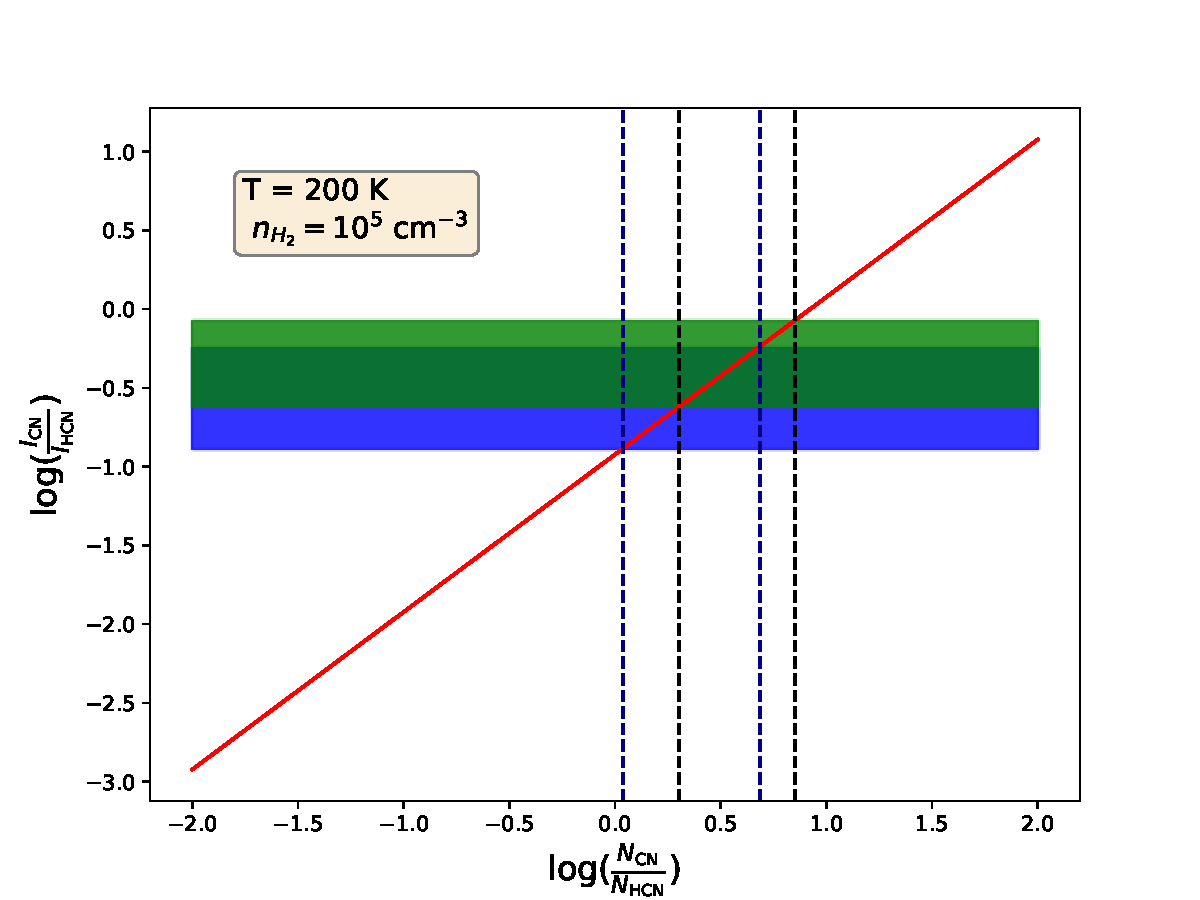
\includegraphics[width=10cm]{RADEX_CN_HCN_200K_1e5.eps}
\caption{The ratio of CN and HCN column densities obtained with RADEX for $n_\mathrm{H} = 10^5$ cm$^{-3}$ and
$T_\mathrm{kin} = 200$ K (red line). The observed line intensity ratio is
shown as a rectangle, with green color corresponding to the values observed at the 
protostar position and blue color for the outflow positions. Column density ranges are marked with black and navy dashed lines for protostars and outflow positions, respectively.} 
\label{model} 
\end{figure}
%=================================================
%=================================================
\begin{table} \caption{Model-dependent column density ratios of CN and HCN}     
 \centering 
  \label{RADEX_Ns}                       
  \begin{tabular}{c c c c} 
  \hline\hline $n_\mathrm{H_2}$ & $T_\mathrm{kin}$ &
log$_{10}$(N(CN)/N(HCN)) &
log$_{10}$(N(CN)/N(HCN)) \\ 
$($cm$^{-3})$ & (K) & protostars & outflows \\ 
\hline 10$^{4}$ & 30 & 0.24-0.79 & -0.02-0.63  \\
 10$^{4}$ & 75 & 0.16-0.71 & -0.10-0.55 \\
  10$^{4}$ & 200 & 0.12-0.67 & -0.14-0.51 \\ 
  10$^{5}$ & 30 & 0.28-0.83 & 0.016-0.67 \\
   10$^{5}$ & 75 & 0.27-0.82 & 0.00-0.65 \\
    10$^{5}$ & 200 & 0.30-0.85 & 0.04-0.69 \\ 
    10$^{6}$ & 30 & 0.38-0.92 & 0.10-0.75 \\ 
    10$^{6}$ & 75 & 0.43-0.98 & 0.16-0.81 \\ 
    10$^{6}$ & 200 & 0.50-1.05 & 0.23-0.88\\
     \hline 
     \end{tabular} 
     \end{table}
%=================================================
Table 3 shows the molecular line ratios at protostar and outflow positions in Serpens 
calculated separately for the fully integrated profiles and for the line wings. 
Here, we will discuss the results for (i) ratios of different isotopologues, informing 
about the line opacities, (ii) the ratio of two transitions of H$^{13}$CN,
indicating gas temperature, (iii) ratios of different species, reflecting 
their relative abundances.

%==============================================================
\subsubsection{Ratios of different isotopologues}
%==============================================================
 
The line ratio of the same transition of two isotopologues can be used a tracer of 
line opacity of the more abundant species, assuming that the emission in the 
other isotopologue is optically thin. We adopt a standard method described in \citep{Gol84} 
to determine the line opacities of HCN 1-0 and CS 3-2 lines, both in the protostar 
and outflow positions. We assume that both isotopologues arise from the 
same physical region, described by the excitation temperature, $T_\mathrm{exc}$, and 
in local thermodynamical equilibrium (LTE). Using the equation \ref{eq1}, we obtain
the values of 0.3-5.7 and 0.3-4.8 for the fully-integrated line profiles of HCN and CS with their isotopologues respectively.
\begin{equation} 
\label{eq1} \frac{T_{\mathrm{HCN}}}{T_{\mathrm{H^{13}CN}}} =
\frac{X[\mathrm{HCN}]}{X[\mathrm{H^{13}CN}]} \frac
{1-\exp(-\tau_{\mathrm{HCN}})}{\tau_{\mathrm{HCN}}} 
\end{equation} 

For comparison, the expected ratio in case of optically emission is 30 and 20 for 
the HCN/H$^{13}$CN \citep{Dan13} and CS/C$^{34}$S \citep{Ter10} ratios, respectively. Thus, 
the emission in both species is optically thick, when the entire profile is considered.
In contrast, the \textbf{HCN/H$^13$CN ratio measured in the line wings is around 10-40 (except Ser-SMM8). It corespond to the optical depth of 0.6-2.6 that is} comparable to the optically thin ratio. \textbf{Similarly, line ratio of CS/C$^{34}$S can be translated to $\tau \approx 0.8-2.6$.} Thus, in the selected velocity ranges the ratios of line emission
is these species are a valuable measure of real emission. 

We note that an alternative method of calculating the line optical depths is to check 
the ratios of various components due to hyperfine splitting. However, for HCN show 
considerable anomalies (\citep{Lou12}. The method can be applied to CN molecular lines based on three the strongest components F=3/2$\rightarrow$1/2, F=5/2$\rightarrow$3/2, F=1/2$\rightarrow$1/2 with ratio of 0.1235:0.3333:0.0988 \citep{Ska83}. The optical depth varies from 0.4 to 1.6 and from 0.2 to 1.0 for protostars and outflows positions, respectively. 

The calculated optical depths are in agreement with the calculations performed using the 
1D radiative-transfer code RADEX \citep{vdT07}. Assuming column density of 
HCN of $3 \times 10^{14}$ cm$^{-2}$, hydrogen density of $10^5$ cm$^{-3}$ and kinetic temperature of
the gas of 50 K, the optical depths of HCN is 4.4.
For CS, the value is 2.1, assuming column density of $5 \times 10^{13}$ cm$^{-2}$. 

%It is seen that both the HCN and CN lines are optically thick so the calculated column densities can
%be underestimated by up the order of magnitude. Nevertheless, while both lines are similarly thick,
%this will have little effect on the relative values of calculated column densities.

%==============================================================
\subsubsection{The H$^{13}$CN 2-1/1-0 ratio}
%==============================================================
The H$^{13}$CN 2-1 emission was detected in two positions only: Ser-SMM4 and Ser-SMM9. The ratio of two lowest transitions is 1.98 and 1.31 respectively. Based on two different transitions of the same molecule, the exitacion temperature can be calculated using Equation \ref{eq2}, where E i refers to energy and n i refers to
population of upper and lower level.
\begin{equation} 
\label{eq2} 
T_{\mathrm{ex}} = \frac{E_u - E_l}{k \ln \frac{n_l}{n_u}} 
\end{equation}

The exitation temperature equals 2.43 K and 2.77 K for Ser-SMM4 and Ser-SMM9 respectively. These values are much lower than expected in the
envelopes and outflows of low-mass protostars, and likely affected by the low signal-to-noise of the detected lines. \textbf{\citealt{Yil13} found the excitation temperatures for Ser-SMM1, Ser-SMM3 and Ser-SMM4 using rotiational diagrams. Based on $^{13}$CO and C$^{18}$O the exitation temperature of the envelope is about 40-60 K. The $^{12}$CO emission in connected with the outflows with kinetic temperature of 70-100 K.}
%\textbf{The gas temperatures found using CO 7-6/ CO 6-5 ratio are 0.86-1.08 for the Ser SMM1, SMM3 and SMM4 (citation?)}

%=================================================
\subsubsection{Ratios of different species}
%=================================================
 
The median value of the CN/HCN ratio at the protostars positions is $0.63 \pm 0.19$. Slightly lower
ratio is calculated for the outflow positions and equals $0.51 \pm 0.20$.
The CN and HCN ratio varies between 0.13 at the Outflow 3 to 0.85 at the Ser-SMM3. 

There is no significant dependence between the CN and HCN ratio and the evolutionary stage of a source. The ratio for the
Class 0 protostars is $0.61 \pm 0.23$ and for the Class I protostars is $0.67 \pm 0.17$.

%=================================================
\section{Analysis}
%=================================================
In this section, we calculate column densities of the molecules with the aid 
of radiative-code RADEX and compare them to the results from the chemical-code Nahoon, 
run for a set of gas temperatures, densities and UV radiation fields. 
%============================================================
\subsection{Column densities of molecules from observations}
%============================================================

In case of optically thin lines and the LTE conditions, the column density of the 
upper level of a given molecule, $N_\mathrm{u}$, can be calculated using the equation \ref{eq3}. 
Here, $\beta$ is a constant equal 1937 cm$^{-2}$, $W$ is the integrated
intensity of the emission line ($\int{T_{mb} \, dV}$), and $\nu$ is a transition 
frequency in GHz. 

In order to calculate the total column density of a given molecule, 
we adopt the gas temperature of 75 K (see \S 3.3.2). Equation \ref{eq4} takes into account the 
temperature-dependent partition function $Q$($T$) for a given molecule, and 
the upper level energies ($E_\mathrm{u}$) and level degeneracies ($g_\mathrm{u}$);
$k$ is a Boltzmann constant. Appendix E shows the results obtained for all observed 
molecules, both for the fully-integrated line profiles and the lines wings.


\begin{equation} 
\label{eq3} N_\mathrm{u} = \beta \, \frac{\nu \,W}{A} 
\end{equation} 
\begin{equation} 
\label{eq4} N_\mathrm{tot} = Q(T_\mathrm{exc}) \, \exp(\frac{E_\mathrm{u}}{k \, T_\mathrm{exc}})  \frac{N_\mathrm{u} }{g_\mathrm{u} } 
\end{equation} 
%The column densities of the upper level of CN $J=1-0$ and HCN $J=1-0$ transitions are presented in
%Table~\ref{table:fluxes}. The lowest transition of CN is more abundant molecule than the lowest
%transition line of HCN at the low-mass protostars positions. The column density of CN $J=1-0$ varies
%between 10$^{14}$ -10$^{15}$ cm$^{-2}$, while in the column density of the HCN’s lowest transition
%reaches 10$^{14}$ cm$^{-2}$. In the case of Ser-SMM2, Ser-SMM3, Ser-SMM4, Ser-SMM6 and Ser-SMM12 HCN
%$J=1-0$ line column density is an order of magnitude lower than the column density of the equivalent
%CN transition. This result provides a clue to better understand of the low-mass protostars
%chemistry.

Because of the optical thickness of HCN (\S 3.3.1), we also employ the non-LTE radiative transfer code RADEX 
to obtain independent determinations of the column densities. In order to mimic the optically thin case,
for the calculations we adopt the HCN column density of 10$^8$ cm$^{-2}$. We vary the column density 
of CN from 10$^6$ cm$^{-2}$ to 10$^{10}$ cm$^{-2}$. The typical physical conditions of the gas 
in low-mass star forming regions are: number densities, $n_\mathrm{H}$ of the order of \textbf{$10^{4}-10^{6}$} cm$^{-3}$ 
and kinetic temperature $T_\mathrm{kin}$ of 30-200 K. Table~\ref{RADEX_Ns} shows the ratios of the calculated 
column densities of CN and HCN for these different sets of parameters, and assuming a line width of 1.0 km s$^{-1}$, for protostars positions and outflows separately.

The models are a means to translate the observed line ratios of CN and HCN into column densities ratios. 
Figure \ref{model} shows \textbf{an example} model calculated for \textbf{200K and $10^{5}$ cm$^{-1}$. Similar models can be found in Fig. \ref{RADEX_models} for} the densities and temperatures typical for 
outflows in low-mass protostars (\citealt{vK09}, \citealt{Yil15}). The observed line intensity ratio (full profile) 
in logarithm is in the range from -0.62 to -0.07 and from -0.87 to -0.24 for protostars and outflow positions, respectively. The corresponding column density ratio is
in the range 0.12 to 1.05 and -0.14 to 0.88. Similar models were calculated for other sets of 
temperatures and densities, and the determined scaling factors between the intensity and column
density ratios show a very weak dependence on the adopted physical parameters. The resulting 
column density ratios of CN and HCN are in order of 1-10. 


%=================================================
\subsection{Theoretical column densities from Nahoon}
%=================================================
\begin{figure} 
\centering 
\includegraphics[width=10cm]{starless.eps} 
\caption{Time evolution of CN
(red line), HCN (blue line) and CS (black line) abundances obtained with Nohoon astrochemical code
with initial parameters of $n_\mathrm{H} = 10^4$ cm$^{-3}$, $T = 10$ K, $A_\mathrm{V}$ =
5 mag. The assumed cosmic-ray ionization rate is $1.3\times10^{17}$ s$^{-1}$, dust to gas mass ratio
is 0.01, dust grain radius is $10^{-5}$ cm, grain density is 3 g cm$^{-3}$.} 
\label{starless}
\end{figure}
%=================================================
%=================================================
\begin{figure} 
\centering 
\includegraphics[width=10cm]{AV5.eps} 
\caption{Contour plot of Nahoon sets
of models of CN/HCN abundances ratio with fixed visual extinction $A_\mathrm{V}$ = 5 mag at the time
of 10$^{7}$ yrs after star formation began in the cloud.} 
\label{AV5} 
\end{figure}
%=================================================
The Nahoon chemical code is used to calculate theoretical column densities of 
molecules for a set of physical conditions and UV field strengths; it is a well-known
\textbf{almost or del(purely gas-phase)} purely gas-phase chemical code for astronomical applications (\citealt{Wak12}). 

The Nahoon solver computes the chemical evolution in time including 489 species
and 6992 gas-phase and gas-grain reactions based on rate coefficients from the Kinetic
Database for Astrochemistry (KIDA) database\footnote{http://kida.obs.u-bordeaux1.fr/}. 
The Nahoon code can model chemistry at a fixed temperature and density (0D modeling),
 as well as at grid of temperature,
density and visual extinction (1D modeling). 

The UV radiation in Nahoon is described through the relation
between visual extinction $A_\mathrm{V}$ and the photodissociation rate coefficient $k$
(equation ~\ref{eq4}). Here, $\mathrm{\alpha}$ and $\mathrm{\gamma}$ are coefficients
 of photodissociation of HCN equal to $1.64\times10^{-9}$ and $3.12$, respectively \citep{Hea17}.

\begin{equation} \label{eq5} 
k = \alpha e^{-\gamma A_\mathrm{V}} 
\end{equation} 

In our analysis, we calculate 1D grid with the latest version of Nahoon code (Nahoon\_kida.uva.2014). 
The evolution of the chemical network starts at the time of a dense cloud formation.
Figure~\ref{starless}) shows a model corresponding to a typical dense cloud with temperature of 10 K
and hydrogen total density of $n_\mathrm{H} = 10^4$ cm$^{-3}$. The chemical composition
of the CN, HCN and CS molecules becomes stable at the time of $10^{7}$ yrs; the HCN abundance is higher
than that of CN. We assume the time of $10^{6}$ yrs as the moment when the star formation starts in
a dense cloud. We use model abundances for all 489 species at this moment of time 
as an input data for the forthcoming set of models.

The closest neighbourhood of low-mass protostars is simulated based on the initial abundances of
all species from starless cloud modelling. We adopt the cosmic-ray ionization
rate of $1.3\times 10^{17}$ s$^{-1}$ \citep{Cra78}. The sets of models are run
for the temperature range between 10 and 200 K and the total hydrogen densities from $10^4$
cm$^{-3}$ to $10^6$ cm$^{-3}$. 

Figure \ref{AV5} show the model results assuming visual extinction of 5 mag \textbf{what corresponds to the} lack 
of UV radiation. In that case, HCN is more abundant than CN by about 2-3
orders of magnitude. The column density ratio of CN and HCN weakly depends on the 
gas temperature, \textbf{so we fix the gas temperature at 50K for envelopes of protostars and 200 K for outflows}.
%=================================================
\begin{figure} 
\centering \includegraphics[width=10cm]{G0_50K_modification.eps} 
\caption{he column ratio of CN and HCN from Nahoon for a 
range of hydrogen densities and UV field strengths assuming $T$ equal 200 K (contours) 
and the observed column density ratios (in green).} 
\label{G0_50} 
\end{figure}
%=================================================
\begin{figure} 
\centering 
\includegraphics[width=10cm]{G0_200K_modification.eps} 
\caption{Similar to Fig.~\ref{G0_50} but for fixed temperature $T = 50$ K.} 
\label{G0_200} 
\end{figure}
%=================================================
%=================================================
\begin{figure} 
\centering 
\includegraphics[width=9cm]{serpens_hcn10_and_cn10.eps}
\caption{Map of the intensity ratio of CN 1-0 (colours) and HCN 1-0
(contours) in Serpens. The labels are the same as in Figure 2. Contour levels start at 30 $\sigma$ with the steps of 20 $\sigma$.
The CN emission has been resampled to beam size of HCN in order to compare the same emitting regions.} 
\label{cn10_and_hcn10} 
\end{figure}
%=================================================
%\begin{figure} 
%\centering 
%\includegraphics[width=10cm]{G0_T.eps} 
%\caption{Similar to Fig.~\ref{AV5}
%but for fixed hydrogen density $n_\mathrm{H} = 10^5$ cm$^{-3}$.} 
%\label{G0} 
%\end{figure}
%=================================================

In the next step, we run the model for the
range of visual extinction between \textbf{-$2.5^{\mathrm{m}}$} and $2.5^{\mathrm{m}}$ that corresponds to
the UV radiation field G$_0$ of $4\times 10^{-4}$ to \textbf{-$2.4\times 10^{3}$}. \textbf{The reaction network was corrected for HCNH$^+$ photodissociation. The HCNH$^+$ can be photodissociated into HCN$^+$ or HNC$^+$ molecules. We estimated the reaction rate coefficient as 10\% of the HCN photodissociation rate.}
\textbf{Figures \ref{G0_50} and \ref{G0_200}
Show} the ratio of CN and HCN \textbf{abundances} as a function of $n_\mathrm{H}$ and G$_0$. The observed ratios 
of 1-10 match the calculated ratios \textbf{in three regimes: for very weak UV fields (<$10^{-3}$ G$_0$),  for the relatively weak UV fields of $10^{-1}-10^1$ and relatively strong UV fields of $10^{2}-10^3$.}
%Thus, the simulations are consistent with the presence of 
%The calculated column density ratio covers parameter
%space of all probed densities and G$_0$ range between $10^{-4}$ and 0.05 in weak UV radiation
%regime. The observed CN/HCN ratio is reproduced at the G$_0$ values greater than $1.5 \times 10^{3}$
%as well. HCN is more abundant than CN in very weak (<$10^{-3}$ G$_0$) radiation fields. This result
%is consistent with simulations of a starless cloud that leads to a conclusion that additional UV
%radiation source is needed to reproduce the observational ratios.

%The sets of models shown in this section indicate that CN/HCN column density ratio covers the range
%of 1-10 regardless of excitation conditions. This result suggests that the UV radiation may play an
%important role around low-mass protostars. 
%
\section{Discussion}
%=================================================
%\subsection{Morphology of the UV-irradiated region}
%=================================================
%=================================================
\subsection{Comparison of the spatial extent of CN and HCN}
%=================================================
The relative abundance of CN and HCN molecules is widely used a tracer of UV radiation in different
astronomical context: reflection nebulae (e.g. \citealt{Fue95}), proto-planetary disks (e.g.
\citealt{Cha12}), proto-brown dwarfs (e.g. \citealt{Ria18}). CN is a product of photodissociation of
HCN with the photodissociation rate of $1.64\times10^{-9}$. CN has smaller photodissociation rate of
$5.19\times10^{-10}$ (\citealt{Hea17}), thus is not that sensitive for photodissociation as HCN.
Since CN and HCN can be photodissociated selectively, therefore the CN/HCN ratio probes regions
affected by UV radiation. The ratio is the highest near the source of the UV emission, and decreases
with the distance from the source (\citealt{Fue93}). 

Figure \ref{cn10_and_hcn10} shows a large-scale map of CN 1-0 and HCN 1-0. 

The CN $J=1-0$ transition is shifted to the north in respect to the HCN $J=1-0$ emission. It is
highly concentrated in the SE subcluster, while the NW subcluster is dominated by the HCN. Both
molecules show a diffusive ‘bridge’ between the two subclusters. It is connected with Ser-SMM4 and
Ser-SMM1 outflows in HCN, while the CN follows the dust continuum emission. The emission in both
molecules is anti-corelated north from Ser-SMM6 and west from Ser-SMM4 sources. At the dense area of
Ser-SMM9 surrounding CN/HCN ratio is significantly weaker.

Both species has been detected in all sources positions. CN as a product of HCN photodissotiation
indicates other properties of low-mass protostars surroundings (Section 4). The highest CN/HCN
integrated intensity ratio occurs in Ser-SMM6 and Ser-SMM3 protostars. On the other hand, Ser-SMM9 object is characterised by very low CN/HCN line ratio.
Similarly low CN/HCN ratio is measured in outflow positions no. 3 and 4.

Most of the sources show high flux values in both molecules (Table~\ref{table:CN/HCN}). However,
they present unequal levels which indicates regions of different properties. The CN/HCN ratio varies
between protostars positions, as well as between off-source positions. \textbf{ del? Repeated information: The highest CN/HCN ratio is
found in Ser-SMM3, Ser-SMM6 and Ser-SMM12 sources}. This parameter seems to be not correlated with the
evolutional stage of a protostar. All the sources with the highest CN/HCN ratio are located in the
SE subcluster. Ser-SMM3 and Ser-SMM6 are situated in close neighbourhood, in the area characterised
by high emission of CN $J=1-0$ line. At Ser-SMM9 and Ser-SMM10 protostars the lowest CN/HCN ratio is
observed. Both sources are young, Class 0 YSOs. In addition they are separated by $\approx 45$
arcsec from the other sources.

\textbf{The same trend can be recognised in the integrated intensity ratio measure in the wings only. The highest ratio is present at the same protostars, although SMM12 shows the highest value in this case. It is located in 60 arcsec form the Ser-SMM3 and Ser-SMM6 protostars, in the area of with significantly lower level of HCN emission. No outflow is known from Ser-SMM12. The CO $J=6-5$ line in the neighbourhood of Ser-SMM12 does not indicate an outflow either. Extremely low CN and HCN ratio in the wings emission is connected with blue-shifted outflow from Ser-SMM4 (outflow position no. 3). In general the ratio is lower at outflow positions than at positions of protostars that indicates the UV radiation is produced in the closest neighbourhood of the protostars. The most prominent emission of the CN line is associated with the protostars concentration in the SE subcluster, rather than with the evolutionary stage of a source.}

%=================================================
\begin{figure} 
\includegraphics[width=10cm]{reactions-mediumG0.eps} 
\caption{Reactions network for UV irradiated gas of G$_0$ = $10^{-1} - 10^{1})$.}
\label{reactions_mediumG0} 
\end{figure}
%=================================================
\begin{figure} 
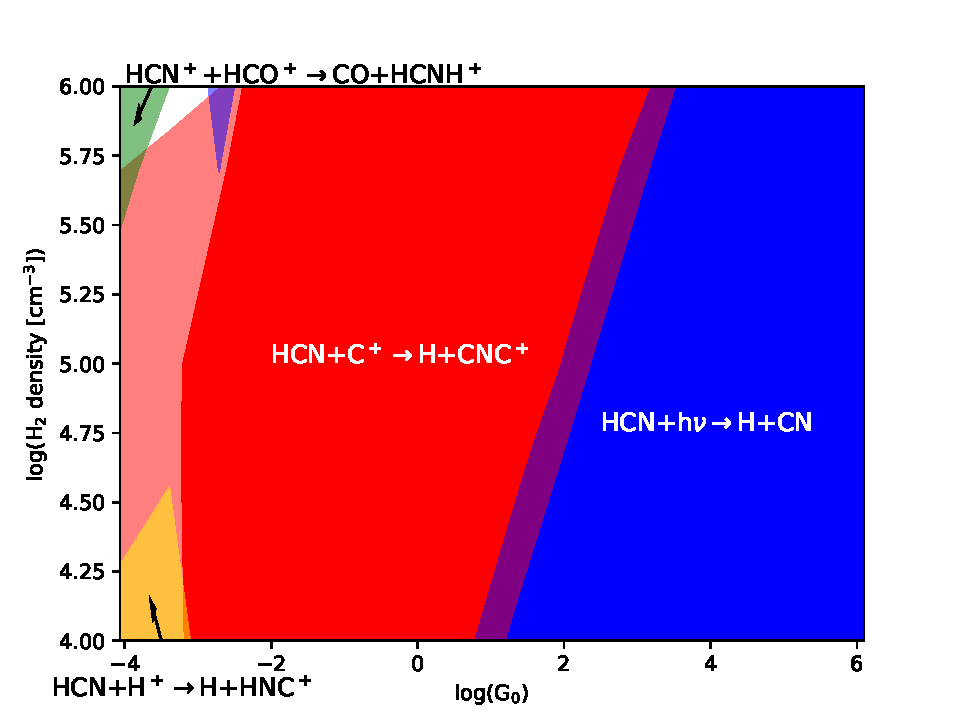
\includegraphics[width=10cm]{destruction_HCN_dominant.eps} 
\caption{Dominant reactions
of HCN destruction. Reactions conributed at least 50$\%$ of total flux are marked with full colous.
Transparent colours correspond to 30$\%$-50$\%$ contribution.} 
\label{HCN_dest} 
\end{figure}
%=================================================
\subsection{UV field strengths in Serpens}
%=================================================
%=================================================
\begin{table*} 
\caption{Dominant processes in CN and HCN chemistry at 50 K}      
\centering       %
\label{reactions_50}    

\begin{tabular}{c c c c} 
\hline\hline 
Molecule & Weak UV fields  & Medium UV fields  & Strong UV fields  \\ 
& (G$_0$ = $10^{-3} - 10^{-1})$ & (G$_0$ = $10^{-1} - 10^{1})$ & (G$_0$ = $10^{1} - 10^{6})$ \\ 
\hline 
\multirow{8}{*}{CN} & \multicolumn{3}{c}{\textbf{Destruction}}\\ 
& O + CN $\rightarrow$ N + CO & CN + ph $\rightarrow$ C + N & CN + ph $\rightarrow$ C + N\\ 
& CN + N $\rightarrow$ C + N$_2$ & O + CN $\rightarrow$ N + CO & \\
\vspace{2.5 pt} &\multicolumn{3}{c}{\textbf{Production}}\\ 
&N + CH $\rightarrow$ H + CN & N + C$_2$ $\rightarrow$ C + CN &  HCN$^+$ + e$^-$ $\rightarrow$ H + CN\\
&CNC$^+$ + e$^-$ $\rightarrow$ C + CN & H + CN$^+$ $\rightarrow$ CN + H$^+$ & N + CH $\rightarrow$ H + CN\\
&N + C$_2$ $\rightarrow$ C + CN &  & H + CN$^+$ $\rightarrow$ CN + H$^+$\\ &  &   & N + C$_2$ $\rightarrow$ C + CN\\
\hline
\multirow{9}{*}{HCN} & \multicolumn{3}{c}{\textbf{Destruction}}\\ 
&HCN + C$^+$ $\rightarrow$ H + CNC$^+$ & HCN + C$^+$ $\rightarrow$ H + CNC$^+$ &  HCN + ph $\rightarrow$ H + CN\\
&HCN$^+$ + HCO$^+$ $\rightarrow$ CO + HCNH$^+$ &HCN + ph $\rightarrow$ H + CN & HCN + C$^+$ $\rightarrow$ H + CNC$^+$\\
&HCN + H$^+$ $\rightarrow$ H + HNC$^+$ &  &  \\
&HCN + ph $\rightarrow$ H + CN &  &  \\
\vspace{2.5 pt} 
&\multicolumn{3}{c}{\textbf{Production}}\\ 
&N + CH$_2$ $\rightarrow$ H + HCN & H + CCN $\rightarrow$ C + HCN & HCNH$^+$ + e$^-$ $\rightarrow$ H + HCN\\
&H + CCN $\rightarrow$ C + HCN & HCNH$^+$ + e$^-$ $\rightarrow$ H + HCN & H + CCN $\rightarrow$ C + HCN\\
&HCNH$^+$ + e$^-$ $\rightarrow$ H + HCN & & \\ 
&C + HNC $\rightarrow$ C + HCN & & \\ 
\hline \end{tabular} 
\end{table*}
%=================================================
%Comparing CN/HCN results with similar plots of CN/CS and CS/HCN ratio (Fig.~\ref{CN/CS} and
%Fig.~\ref{CS/HCN} respectively) restricts the parameter space to very low-density and weakly
%irradiated gas or a dense gas with strong UV radiation. CN/CS ratio varies between 9 and 29 for the
%all protostars positions, while CS/HCN ratio is in range of 0.12-0.26. Astrochemical models computed
%for these molecules show similar behaviour to that presented for CN/HCN ratio. UV radiation with the
%strength of G$_0$ in order of $10^{3}-10^{4}$ is not very probable in low-mass protostars
%neighbourhood. At the protostars' positions high hydrogen densities can be assumed. Astronomical
%models show that an additional UV radiation source of the strength of few hundredth of the average
%interstellar UV radiation field is required to cover the observational ratios.

Low CN/HCN ratio found in astrochemical model for strongly irradiated gas is a surprising result.
Both production and destruction of each molecule need to be investigated in order to explain the
reason behind HCN abundances being higher than expected. Detailed models of the most dominant
reactions for destruction and production of each molecule are presented in Fig. ~\ref{CN_dest} –
Fig.~\ref{HCN_prod} with the assumption of fixed 50 K temperature. Reaction flux is defined as
reactants abundances multiplied by reaction rate coefficient. Only these reactions were taken into
consideration which accumulated flux is greater than 80$\%$ of the total flux of all reactions
contributed in the studied molecules destruction or production.

The reactions distribution in the parameter space is not very strongly depended on hydrogen
densities. The strength of an additional UV radiation source is the parameter that distinguishes the
dominant reactions the most. It was divided into three regimes: with weak, intermediate and strong
UV field. The reactions where CN or HCN production or destruction is greater than 30$\%$ are listed
in Tab.~\ref{reactions_50} as well as illustrated in \textbf{Fig.~\ref{reactions_mediumG0}, as well as in Fig.~\ref{reactions_smallG0}-
Fig.~\ref{reactions_largeG0}.}

In the regime of weak UV radiation fields dominant formation channels of CN and HCN are hydrocarbons
(CH and CH$_2$ respectively) reactions with atomic nitrogen. In more dense areas electron reaction
with CNC cation plays role in the CN formation. The destruction of CN is mostly dominated with
reaction with neutral oxygen (60-70$\%$) or nitrogen (30$\%$ or less). In weakly irradiated
environment atomic elements are more abundant in the neutral state. More of the ionised atoms are
produced with the increase of the UV radiation what blocks these effective channels of CN
destruction.

On the other hand, HCN destruction is driven by many channels in the weakest UV regime. Simultaneous
impact of few different reactions is not as effective as the reaction ruling the CN destruction. It
leads to higher HCN abundances compared to CN. HCN reaction with abundant C+ is the dominant
destructive reaction for slightly stronger radiation fields (>$10^{-3}$). This reaction results in
CNC+ production which quickly reacts with electron forming CN. That explains why CN/HCN ratio
increases with larger radiation.

CN/HCN ratio is widely used as UV radiation tracer in PDRs (eg. \citealt{Thi04}, \citealt{Han15}).
HCN photodissociates into CN molecule and H atom, while CN requires more energetic photon (> 12.4
eV) to be disintegrated (\citealt{vDi87}). This leads to higher abundance of CN molecules and
increases CN/HCN column density ratio. Fluxes of HCN photodissociation (Fig.~\ref{HCN_dest}) show
that this reaction has marginal contribution in nitrogen chemistry up to G$_0$ $\approx$ 100.

%=================================================
\subsection{Comparisons to the results from \textit{Herschel}}
%=================================================

\begin{table*} 
\caption{Comparison of different line ratios}      
\centering       %
\label{line_ratios}    

\begin{tabular}{l c c c c c c} 
\hline\hline 
Lines & SMM1  & SMM3r  & SMM3c & SMM3b & SMM4b & Ref. \\ 
\hline 
[OI](63$\mu$m) / o-H$_2$O(179$\mu$m) & 8.58 & 1.31 & 2.60 & 2.21 & 2.19 & 1, 2 \\ 
OH(84$\mu$m) / o-H$_2$O(179$\mu$m) & 0.96 & 0.13 & 0.23 & 0.16 & 0.10 & 1, 2 \\ 
\mbox{[OI](63$\mu$m)} / OH(84$\mu$m) & 8.98 & 9.76 & 11.39 & 13.69 & 22.17 & 1, 2 \\
CH$^+$(1-0) / OH$^+$(1-0) & 0.70 & - & - & - & - & 3\\ 
OH$^+$(1-0) / o-H$_2$O$^+$(1-0) & $\geq$15.96 & - & - & - & -& 3\\
C$^+$ / CH$^+$(1-0) & 0.16 & - & - & - & -& 3\\
CN(1-0) / HCN(1-0) & 0.61 & 0.79 & 0.85 & 0.86 & 0.46 & This work\\
\hline \end{tabular} 
\tablebib{(1)~\citet{Goi12};
(2) \citet{Dio13}; (3) \citet{Ben16}.
}
\end{table*}

%=================================================

Previous studies of energetic processes around low-mass protostars showed observational premises of
the influence of UV radiation on molecules. These works focused on intermediate-\textit{J} CO
transitions (up to 6-5) that traces gas with the kinetic temperature around 100 K. With the Water in
Star-Forming Regions with the Herschel Space Observatory (WISH) project (\citealt{vDi11}) higher CO
rotational transitions (up to 49-48) were studied that provided information of two temperature
components seen in molecular outflows: warm with $T_\mathrm{rot} \approx 300$ K and hot with
$T_\mathrm{rot} \approx 600-800$ K (\citealt{Kar13}, \citealt{Gre13}). The observations of the water
molecule shows a broad and medium-broad components associated with non-dissociative \textit{C}
shocks and dissociative \textit{J} shocks respectively (\citealt{Kri13}, \citealt{Mot14}). These
spectral components can be correlated to the CO rotational temperature components (\citealt{Kri17}).
Another tracers sensitive to UV radiation, ionised hydrides such as CH$^+$, OH$^+$ and H$_2$O$^+$,
were found in outflow cavities (\citealt{Ben16}). The UV fluxes were estimated as 10$^2$-10$^3$
higher than average interstellar radiation. There is no molecular evidence for influence of X-rays
for chemical compositions of low-mass protostars.

Most of the low-mass protostars have a broad, centered on $v_{\mathrm{source}}$ CO $J=16-15$ and
H$_2$O component in their spectra (\citealt{Kri17}). There are typically $\approx 20$ km s$^{-1}$
broad and associated with cavity shocks. The emitting gas is located in shocks along the outflow
cavity wall or along the molecular wind alternatively (\citealt{Yva16}). Some of the sources show a
narrow, offset component as well that is seen in the PACS CO ladder with $T_\mathrm{rot} \approx
600-800$. The gas dissociated by UV photons and carried out form the protostar was proposed as an
origin of the pre-shock gas (\citealt{Kri17}). Thus, ultraviolet radiation can propagate in large
scales of 1000 AU from the central protostar, changing the properties of the surrounding matter. The
hypothesis of the UV irradiated shocks is raised also based on H$_2$O/OH ratio observations. The
ratio showed a few order of magnitude disagreement with fully-shielded shock models
(\citealt{Kar14}). The observations are reproduced with predictions of \textit{C}-shock models
illuminated by UV photons of the strength 0.1-10 times the interstellar value (\citealt{Mel15}). The
other photodissociation tracers, fluxes of [OI] and [CII] are significantly higher than predicted by
fully-shielded \textit{C}-shock models (\citealt{Kar18}). Therefore, ultraviolet radiation may play
an important role in low-mass protostars surroundings.

%=================================================
\section{Conclusions}
%=================================================
IRAM 30~m / EMIR observations of CN and HCN emission pin-point the location 
of the impact of UV radiation on the chemistry of low-mass star forming region in Serpens. 
A combination of simple models using radiative-code RADEX and chemical code Nahoon 
allows us to determine physical conditions of the gas, column densities of molecular species,
 and estimate the UV radiation field strength. The main conclusions of our study are the 
 following. 
%=================================================
\begin{itemize} 
\item The spatial extent of HCN 1-0 and CN 1-0 show significant differences, with 
HCN resembling the CO 6-5 emission tracing outflows and CN concentrated close to the 
individual protostar positions or their groups.
\item The ratios of CN and HCN systematically differ between protostar and outflow position,
both taking into account the integrated line profile and the line wings \textbf{[TBC!]}. The ratio 
is the highest at the positions of the protostars, confirming the impact of UV identified 
using \textit{Herschel} as part of the WISH program. 
\item For typical densities of low-mass protostellar envelopes of $10^5$ cm$^{-3}$ and 
gas temperatures of $75$ K \textbf{(TBC)}, the chemical network for nitrogen-species is sensitive 
to UV photons. The ratio of CN and HCN is primarily driven by the UV photodissociation of HCN into CN 
in a broad range of UV field strength. The tracer is most useful for G$_\mathrm{0}>10^{2}$. 
\item The column density ratios of CN and HCN equals 1-10, which corresponds to G$_0$ $\approx$ $10^{-2}$. 
These values are in agreement with, yet in the lower end of the UV field strength obtained using 
H$_2$O and OH ratios from \textit{Herschel}.
\end{itemize}

Similar observations for a larger sample of sources is needed to fully exploit 
the impact of UV radiation on the physical and chemical conditions in low-mass star 
forming regions. Detailed 3D modelling of protostellar envelopes with outflow cavities 
is necessary to fully constrain the strengths of the UV fields in physical components 
of young stellar objects.

\begin{acknowledgements} AM, AK, MG and MŻ acknowledge support from the Polish National Science
 Center grant 2016/21/D/ST9/01098. AK acknowledges support from the First TEAM grant of 
 the Foundation for Polish Science No. POIR.04.04.00-00-5D21/18-00 and the hospitality 
 of the StarPlan group in the University of Copenhagen during the manuscript preparation.
Support for this work was provided by the Polish National Agency for Academic Exchange through the project InterAPS.
This research has made use of data from the Herschel Gould Belt survey (HGBS) project
(http://gouldbelt-herschel.cea.fr). The HGBS is a Herschel Key Programme jointly carried out by
SPIRE Specialist Astronomy Group 3 (SAG 3), scientists of several institutes in the PACS Consortium
(CEA Saclay, INAF-IFSI Rome and INAF-Arcetri, KU Leuven, MPIA Heidelberg), and scientists of the
Herschel Science Center (HSC). 
\end{acknowledgements}


% WARNING
%-------------------------------------------------------------------
% Please note that we have included the references to the file aa.dem in order to compile it, but we
% ask you to:
% %
% - use BibTeX with the regular commands:
\bibliographystyle{aa} % style aa.bst 
\bibliography{amirocha} % your references Yourfile.bib

%
% - join the .bib files when you upload your source files
%-------------------------------------------------------------------
%
\begin{appendix} %First appendix 
\section{Spectral Energy Distributions}

Broad-band observations are needed in order to determine physical properties of a protostar. Dunham
et al. 2015 studied properties of protostars in the Serpens molecular cloud using 2MASS
(\citealt{Skr06}) and Spitzer IRAC/MIPS (\citealt{Eva09}), observations covering the range of
1.25–70 $\mu$m, photometry from Wide-field Infrared Survey Explorer 12 and 22 $\mu$m (WISE;
\citealt{Wri10}), SHARC-II 350 $\mu$m (\citealt{Sur16}), the SCUBA Legacy Catalog 450 and 850 $\mu$m
(\citealt{dFr08}) and 1.1 mm observations from Bolocam dust survey (\citealt{Eno07}). The Serpens
Main region was also observed during the Herschel Gould Belt survey project (\citealt{And10}) at 70, 160, 250, 350 and 500 $\mu$m.
SPIRE/PACS photometry in the Serpens molecular cloud is discussed in Fiorellino et al. (in prep.). The flux densites used in the SED analysis are in Tab.~\ref{SED_data}.

Based on SEDs the bolometric temperature and luminosity can be calculated for each of the observed
protostars. The bolometric luminosity was determined by integrating the SEDs over frequency:
\begin{equation} \label{eq6} L_{bol} = \pi \, d^2 \, \int F_\nu d\nu \end{equation} where $d$ is the
cloud distance of $436 \pm 9.2$ pc (\citealt{Ort17}). The bolometric temperature was calculating as
described in \citealt{Mye93}: \begin{equation} \label{eq7} T_{bol} = 1.25 \, 10^{-11} \, \bar{\nu}
\end{equation} where $\bar{\nu}$ is the mean frequency given by: \begin{equation} \label{eq8}
\bar{\nu} = \frac{\int \nu F_\nu d\nu}{ \int F_\nu d\nu} \end{equation}

Using Scipy \textit{splrep} and \textit{splev} functions cubic smooth spline interpolation of the
photometric data was performed while calculating the protostars parameters. Integration along the
resulting axis was obtain with the composite trapezoidal rule (\textit{Scipy} package). The
photometric data allows us to perform the integration along wide range of wavelength with exception
of SMM8. Here we have only 4 photometric points from the Herschel Gould Belt so the calculeted
bolometric luminosity and temperature can be underestimated.

\begin{figure} 
\includegraphics[width=8cm]{serpens_seds.eps} 
\caption{Spectral Energy Distributions of protostars in the Serpens Main region.} 
\label{seds} 
\end{figure}

\begin{table*} 
\caption{Flux densities in Jy, corrected for the beam size.}      
\centering       %
\label{SED_data}    

\begin{tabular}{l c c c c c c c c c} 
\hline 
$\lambda$ & SMM1  & SMM2  & SMM3 & SMM4 & SMM5  & SMM6 & SMM9 & SMM10 & SMM12 \\ 
($\mu$m) &  &  &  & & & & & & \\ 
\hline 
1.25 &- &- &- & 6.0$\times$10$^{-4}$ & 3.0$\times$10$^{-4}$ & 2.1$\times$10$^{-2}$ &- &- &-\\
1.65 &- &- &- & 3.2$\times$10$^{-3}$ & 9.0$\times$10$^{-4}$ & 2.1$\times$10$^{-1}$ &- &- &-\\
2.17 & -& -& -& 1.0$\times$10$^{-2}$ & 4.3$\times$10$^{-3}$ & 1.0$\times$10$^{0}$ & -&- &-\\
3.6 & 9.0$\times$10$^{-4}$ & 4.0$\times$10$^{-4}$ & 2.8$\times$10$^{-3}$ & 2.4$\times$10$^{-2}$ & 3.1$\times$10$^{-2}$ & 2.5$\times$10$^{0}$ & 2.0$\times$10$^{-3}$ & 7.4$\times$10$^{-3}$ & 2.8$\times$10$^{-3}$\\ 
4.5 & 2.6$\times$10$^{-3}$ & 1.2$\times$10$^{-3}$ & 5.8$\times$10$^{-3}$ & 3.3$\times$10$^{-2}$ & 7.3$\times$10$^{-2}$ & 3.0$\times$10$^{0}$ & 7.0$\times$10$^{-3}$ & 3.3$\times$10$^{-2}$ & 3.0$\times$10$^{-2}$\\ 
5.8 & 2.3$\times$10$^{-3}$ & 2.1$\times$10$^{-3}$ & 7.8$\times$10$^{-3}$ & 4.1$\times$10$^{-2}$ & 1.4$\times$10$^{-1}$ & 5.1$\times$10$^{0}$ & 1.2$\times$10$^{-2}$ & 4.1$\times$10$^{-2}$ & 1.0$\times$10$^{-1}$\\
8.0 & 3.5$\times$10$^{-3}$ & 3.5$\times$10$^{-3}$ & 3.6$\times$10$^{-2}$ & 5.6$\times$10$^{-2}$ & 2.1$\times$10$^{-1}$ & 5.4$\times$10$^{0}$ & 1.7$\times$10$^{-2}$ & - & 2.0$\times$10$^{-1}$\\ 
12.0 & 6.2$\times$10$^{-3}$ & - & - &- & 1.8$\times$10$^{-1}$ & 7.6$\times$10$^{0}$ & 1.2$\times$10$^{-2}$ & 3.8$\times$10$^{-2}$ & 2.2$\times$10$^{-1}$\\ 
22.0 & 1.0$\times$10$^{0}$ & - & - & -& 9.5$\times$10$^{-1}$ & 1.0$\times$10$^{1}$ & 2.1$\times$10$^{-1}$ & 8.0$\times$10$^{-1}$ & 3.1$\times$10$^{0}$\\ 
24.0 & 1.2$\times$10$^{0}$ & 1.0$\times$10$^{-1}$ & 1.1$\times$10$^{-1}$ & 2.8$\times$10$^{-1}$ & 9.9$\times$10$^{-1}$ &- & 2.2$\times$10$^{-1}$ & 1.6$\times$10$^{0}$ & 2.6$\times$10$^{0}$\\
70.0 & 1.4$\times$10$^{2}$ & 3.9$\times$10$^{0}$ & 6.8$\times$10$^{0}$ & - & 8.5$\times$10$^{0}$ & 2.6$\times$10$^{1}$ & 1.2$\times$10$^{1}$ & 8.8$\times$10$^{0}$ & 3.3$\times$10$^{0}$\\
160.0 & 4.7$\times$10$^{2}$ & 2.3$\times$10$^{1}$ & 4.4$\times$10$^{1}$ & 1.9$\times$10$^{1}$ & 1.8$\times$10$^{0}$ & 3.1$\times$10$^{1}$ & 7.5$\times$10$^{1}$ & 1.4$\times$10$^{1}$ & 2.0$\times$10$^{1}$\\
250.0 &  2.4$\times$10$^{2}$ & 2.6$\times$10$^{1}$ & 4.2$\times$10$^{1}$ & 4.6$\times$10$^{1}$ & 4.0$\times$10$^{0}$ & 2.9$\times$10$^{1}$ & 2.5$\times$10$^{1}$ & 6.9$\times$10$^{0}$ & 3.2$\times$10$^{1}$\\
350 & 1.2$\times$10$^{2}$ & 2.4$\times$10$^{1}$ & 3.1$\times$10$^{1}$ & 4.2$\times$10$^{1}$ & 1.6$\times$10$^{1}$ & 1.6$\times$10$^{1}$ & 1.6$\times$10$^{1}$ & 6.5$\times$10$^{0}$ & 3.1$\times$10$^{1}$\\
450.0 & 1.0$\times$10$^{2}$ &-  & 3.1$\times$10$^{1}$ &- &- &- &- &- &-\\
500 & 5.0$\times$10$^{1}$ & 1.7$\times$10$^{1}$ & 1.6$\times$10$^{1}$ & 2.8$\times$10$^{1}$ & 1.2$\times$10$^{1}$ & 9.5$\times$10$^{0}$ & 1.6$\times$10$^{1}$ & 5.1$\times$10$^{0}$ & 1.6$\times$10$^{1}$\\
850.0 & 1.5$\times$10$^{1}$ & 8.9$\times$10$^{0}$ & 8.9$\times$10$^{0}$ & - & 3.9$\times$10$^{0}$ & - & 1.3$\times$10$^{1}$ & 3.0$\times$10$^{0}$ &\\
1100.0 & 6.5$\times$10$^{0}$ & 2.1$\times$10$^{0}$ & 2.1$\times$10$^{0}$ & - & 1.5$\times$10$^{0}$ & 1.6$\times$10$^{0}$ & 3.0$\times$10$^{0}$ & 1.0$\times$10$^{0}$ & 2.1$\times$10$^{0}$\\
\hline \end{tabular} 
\end{table*}

\section{Maps in additional tracers}

\textbf{IRAM 30m spectral line maps in HCN and CS isotopologues are presented in Fig.~\ref{h13cn10} and Fig.~\ref{c34s32}. The H$^{13}$CN $J=1-0$ emission is a sum of all hyperfine splitting components. The H$^{13}$CN $J=1-0$ is spatially consistent with HCN $J=1-0$, although a few times weaker. It peaks around Ser-SMM2, Ser-SMM4 and Ser-SMM9, as well as at the Outflow position no.~3. Except for the Ser-SMM2 protostar, the peaks in H$^{13}$CN are co-spatial with the HCN emission peaks. The emission of H$^{13}$CN $J=1-0$ line is similarly strong in the SE and NW regions of the map.}

\textbf{The C$^{34}$S $J=3-2$ line does not show such extended emission, although it was detected in all outflow positions. The emission is concentrated mostly near Ser-SMM1, Ser-SMM4 and Ser-SMM9 sources, unlike the CS $J=3-2$ which is not that significant around Ser-SMM1. The isotopologues trace the same gas as their regular counterparts.}

\begin{figure} \includegraphics[width=8cm]{serpens_h13cn10.eps} \caption{Similar to Fig.~\ref{iram_maps}
but the emission of the H$^{13}$CN $J=1-0$ line. The first contour at 10 $\sigma$ level, with step
of 10 $\sigma$} \label{h13cn10} \end{figure}


\begin{figure} \includegraphics[width=8cm]{serpens_c34s32.eps} \caption{Similar to Fig.~\ref{iram_maps}
but the emission of the C$^{34}$S $J=3-2$ line. The first contour at 30 $\sigma$ level, with step of
10 $\sigma$} \label{c34s32} \end{figure}

\section{Molecular line profiles}

\textbf{The targeted lines were detected in most of the protostars and outflow positions. Fig.~\ref{Spectra_all} shows the spectra in C$^{34}$S $J=3-2$ , CS $J=3-2$,  H$^{13}$CN $J=2-1$, H$^{13}$CN $J=1-0$, HCN $J=1-0$ and CN $J=1-0$  lines obtained with the IRAM 30m, as well as profiles in CO $J=6-5$ observed with APEX-CHAMP$^+$. The spectra at the Ser-SMM4 position are shown in Fig.~\ref{spectra}. The H$^{13}$CN $J=2-1$ line was detected only at Ser-SMM4 and Ser-SMM9 sources. The Ser-SMM8 protostar is outside of the mapping area in CO $J=6-5$.}



\begin{figure*} 
\centering 
\includegraphics[width=15cm]{serpens_spectra_1.eps}
\label{Spectra1} 
\end{figure*} 

\begin{figure*} 
\centering
\includegraphics[width=15cm]{serpens_spectra_2.eps} 
\label{Spectra2} 
\end{figure*}

\begin{figure*}
\centering 
\includegraphics[width=15cm]{serpens_spectra_3.eps}
\label{Spectra3} 
\end{figure*} 

\begin{figure*}
\centering 
\includegraphics[width=15cm]{serpens_spectra_4.eps}
\label{Spectra4} 
\end{figure*}

\begin{figure*} 
\centering
\includegraphics[width=15cm]{serpens_spectra_5.eps} 
\caption{Serpens Main sources spectra of CO(6-5), C$^{34}$S(3-2), CS(3-2), H$^{13}$CN(2-1), H$^{13}$CN(1-0),
 HCN(1-0) and CN(1-0) lines.} 
 \label{Spectra_all}
\end{figure*}

\section{Line fluxes \textbf{and observed column densities}}

\textbf{Table~\ref{table:fluxes} lists the observed lines and their properties calculated at protostars positions. The integrated intensity $T_{\mathrm{mb}} \, dV$ of a line is measured at 3$\sigma$ level for each spectrum separately. The peak temperature $T_\mathrm{peak}$ is the value at the maximum of a line or of the strongest hyperfine component. Column densities at the upper lever $N_\mathrm{up}$ and total column densities $N_\mathrm{tot}$ were calculated as described in \S 4.1 (Eq.~\ref{eq3} and Eq.~\ref{eq4}).}

\begin{sidewaystable*}
\caption{Integrated fluxes of the observed line at the positions of protostars}\label{table:fluxes}
\centering
\begin{tabular}{l l c c c c c c c c c c} 
\hline\hline             
Line &  & SMM1 & SMM2 & SMM3 & SMM4 & SMM5 & SMM6 & SMM8 & SMM9 & SMM10 & SMM12 \\
\hline \multirow{4}{*}{CN 1-0} & $\int{T_{\mathrm{mb}} \, dV}$ (K km/s) & 6.29 & 8.52 & 12.16 & 10.22 & 2.72 & 10.62 & 2.97 & 4.90 & 2.96 & 10.06 \\
& $T_\mathrm{peak}$ (K) & 0.89 & 1.92 & 3.42 & 1.90 & 0.94 & 3.17 & 0.94 & 0.84 & 0.78 & 1.85 \\
& $N_\mathrm{up}$ (cm$^{-2}$) & 1.3$\times$10$^{13}$ & 1.8$\times$10$^{13}$ & 2.6$\times$10$^{13}$ & 2.2$\times$10$^{13}$ & 5.7$\times$10$^{12}$ & 2.2$\times$10$^{13}$ & 6.2$\times$10$^{12}$ & 1.0$\times$10$^{13}$ & 6.2$\times$10$^{12}$ & 2.1$\times$10$^{13}$ \\
& $N_\mathrm{tot}$ (cm$^{-2}$) & 7.9$\times$10$^{14}$ & 1.1$\times$10$^{15}$ & 1.5$\times$10$^{15}$ & 1.3$\times$10$^{15}$ & 3.4$\times$10$^{14}$ & 1.3$\times$10$^{15}$ & 3.7$\times$10$^{14}$ & 6.2$\times$10$^{14}$ & 3.7$\times$10$^{14}$ & 1.3$\times$10$^{15}$\\

\multirow{4}{*}{HCN 1-0} & $\int{T_{\mathrm{mb}} \, dV}$ (K km/s) & 10.34 & 13.08 & 14.36 & 21.67 & 4.04 & 13.10 & 6.84 & 20.68 & 7.26 & 14.24 \\
& $T_\mathrm{peak}$ (K) & 1.76 & 3.48 & 4.95 & 4.69 & 1.72 & 5.15 & 1.72 & 2.40 & 1.75 & 3.50 \\
& $N_\mathrm{up}$ (cm$^{-2}$) & 6.5$\times$10$^{12}$ & 8.3$\times$10$^{12}$ & 9.1$\times$10$^{12}$ & 1.4$\times$10$^{13}$ & 2.6$\times$10$^{12}$ & 8.3$\times$10$^{12}$ & 4.3$\times$10$^{12}$ & 1.3$\times$10$^{13}$ & 4.6$\times$10$^{12}$ & 9.0$\times$10$^{12}$ \\
& $N_\mathrm{tot}$ (cm$^{-2}$) & 2.5$\times$10$^{14}$ & 3.1$\times$10$^{14}$ & 3.4$\times$10$^{14}$ & 5.2$\times$10$^{14}$ & 9.6$\times$10$^{13}$ & 3.1$\times$10$^{14}$ & 1.6$\times$10$^{14}$ & 4.9$\times$10$^{14}$ & 1.7$\times$10$^{14}$ & 3.4$\times$10$^{14}$\\

\multirow{4}{*}{CS 3-2} & $\int{T_{\mathrm{mb}} \, dV}$ (K km/s) & 5.89 & 8.56 & 8.30 & 14.76 & 2.56 & 8.50 & 4.51 & 12.43 & 3.58 & 9.88 \\
& $T_\mathrm{peak}$ (K) & 1.57 & 3.10 & 2.90 & 4.30 & 1.48 & 3.2 & 2.08 & 2.70 & 1.43 & 3.26 \\
& $N_\mathrm{up}$ (cm$^{-2}$) & 4.1$\times$10$^{12}$ & 5.9$\times$10$^{12}$ & 5.7$\times$10$^{12}$ & 1.0$\times$10$^{13}$ & 1.8$\times$10$^{12}$ & 5.7$\times$10$^{12}$ & 3.1$\times$10$^{12}$ & 8.6$\times$10$^{12}$ & 2.5$\times$10$^{12}$ & 6.8$\times$10$^{12}$ \\
& $N_\mathrm{tot}$ (cm$^{-2}$) & 4.5$\times$10$^{13}$ & 6.5$\times$10$^{13}$ & 6.3$\times$10$^{13}$ & 1.1$\times$10$^{14}$ & 2.0$\times$10$^{13}$ & 6.5$\times$10$^{13}$ & 3.4$\times$10$^{13}$ & 9.5$\times$10$^{13}$ & 2.7$\times$10$^{13}$ & 7.5$\times$10$^{13}$\\

\multirow{4}{*}{C$^{34}$S 3-2} & $\int{T_{\mathrm{mb}} \, dV}$ (K km/s) & 1.27 & 0.86 & 0.50 & 1.49 & 0.32 & 0.76 & 0.26 & 1.83 & 0.39 & 0.56 \\
& $T_\mathrm{peak}$ (K) & 0.56 & 0.47 & 0.36 & 0.64 & 0.42 & 0.56 & 0.35 & 0.62 & 0.40 & 0.42 \\
& $N_\mathrm{up}$ (cm$^{-2}$) & 7.1$\times$10$^{11}$ & 4.8$\times$10$^{11}$ & 2.8$\times$10$^{11}$ & 8.4$\times$10$^{11}$ & 1.8$\times$10$^{11}$ & 4.3$\times$10$^{11}$ & 1.4$\times$10$^{11}$ & 1.0$\times$10$^{12}$ & 2.2$\times$10$^{11}$ & 3.1$\times$10$^{11}$ \\
& $N_\mathrm{tot}$ (cm$^{-2}$) & 7.9$\times$10$^{12}$ & 5.4$\times$10$^{12}$ & 3.1$\times$10$^{12}$ & 9.4$\times$10$^{12}$ & 2.0$\times$10$^{12}$ & 4.8$\times$10$^{12}$ & 1.6$\times$10$^{12}$ & 1.2$\times$10$^{13}$ & 2.5$\times$10$^{12}$ & 3.5$\times$10$^{12}$\\

\multirow{4}{*}{H$^{13}$CN 1-0} & $\int{T_{\mathrm{mb}} \, dV}$ (K km/s) & 1.59 & 1.50 & 0.55 & 1.61 & 0.77 & 0.87 & 0.14 & 2.37 & 1.04 & 1.61 \\
& $T_\mathrm{peak}$ (K) & 0.45 & 0.64 & 0.41 & 0.61 & 0.42 & 0.40 & 0.21 & 0.38 & 0.45 & 0.46 \\
& $N_\mathrm{up}$ (cm$^{-2}$) & 3.3$\times$10$^{11}$ & 3.1$\times$10$^{11}$ & 1.6$\times$10$^{11}$ & 3.4$\times$10$^{11}$ & 1.6$\times$10$^{11}$ & 1.8$\times$10$^{11}$ & 2.9$\times$10$^{10}$ & 5.0$\times$10$^{11}$ & 2.2$\times$10$^{11}$ & 3.4$\times$10$^{11}$ \\
& $N_\mathrm{tot}$ (cm$^{-2}$) & 1.3$\times$10$^{13}$ & 1.2$\times$10$^{13}$ & 4.5$\times$10$^{12}$ & 1.3$\times$10$^{13}$ & 6.2$\times$10$^{12}$ & 7.0$\times$10$^{12}$ & 1.1$\times$10$^{12}$ & 1.9$\times$10$^{13}$ & 8.4$\times$10$^{12}$ & 1.3$\times$10$^{13}$\\

\hline\hline
\end{tabular}
\end{sidewaystable*}

\section{RADEX models}

\textbf{RADEX models predictions for hydrogen densities ranged $10^{4}-10^{6}$ cm$^{-3}$ and kinetic temperature of a gas of 30 – 200 K are presented in Fig.~\ref{RADEX_models}. CN and HCN column densities ratios inferred by the models comparison with observations (blue and green rectangles) are shown in Tab.~\ref{RADEX_Ns}.}

\begin{figure*}
\centering 
\begin{subfigure}{.45\textwidth} 
\label{model1} 
\centering
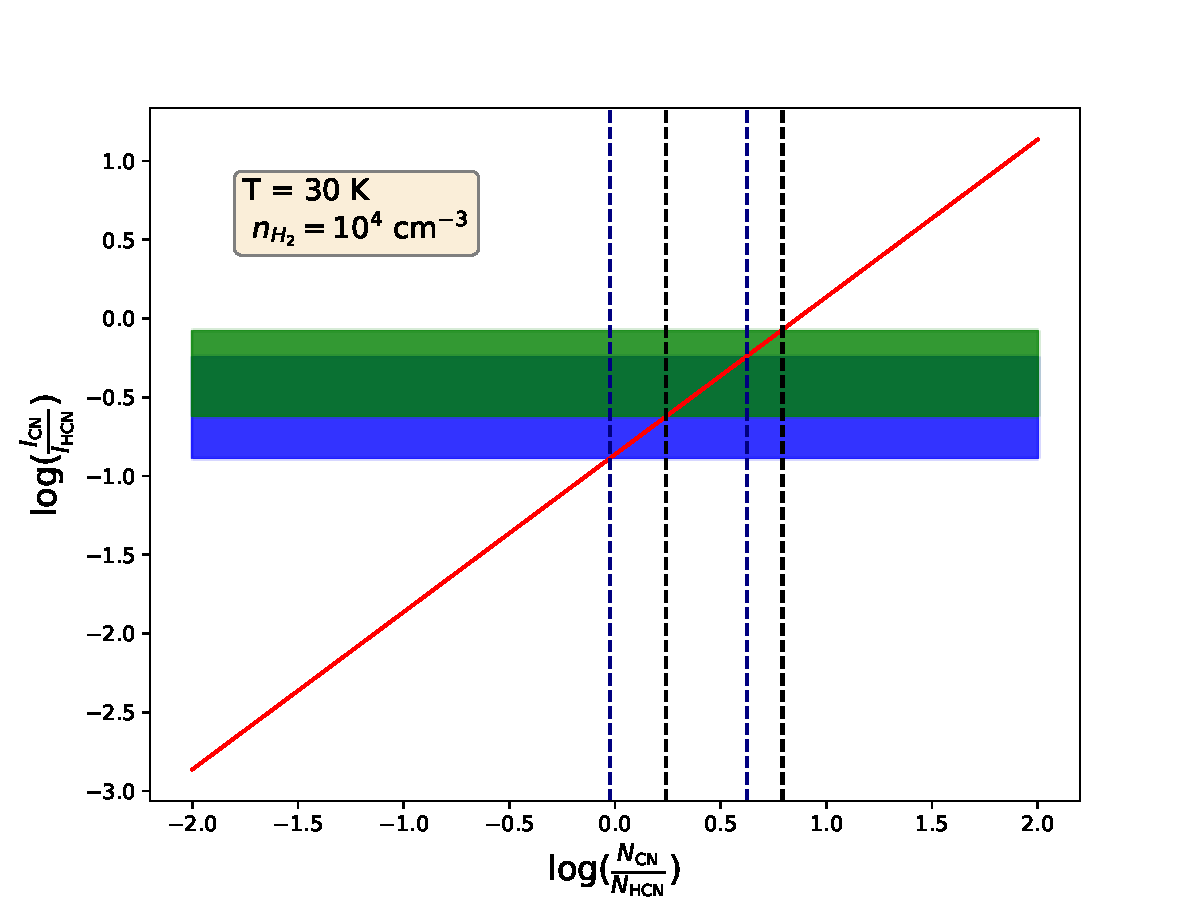
\includegraphics[width=1.\linewidth]{RADEX_CN_HCN_30K_1e4.eps} 
%\caption{} 
\end{subfigure}
\begin{subfigure}{.45\textwidth} 
\label{model2} 
\centering
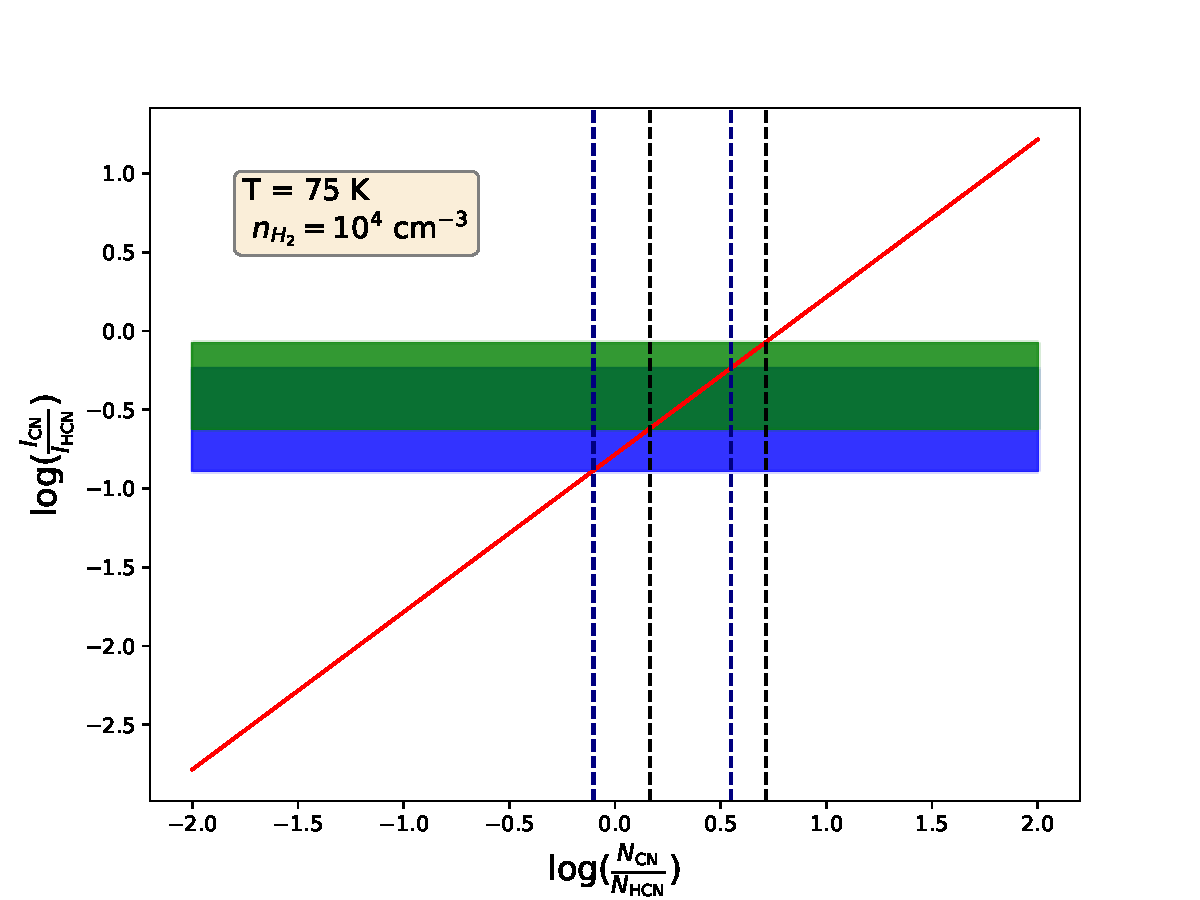
\includegraphics[width=1.\linewidth]{RADEX_CN_HCN_75K_1e4.eps} 
%\caption{} 
\end{subfigure}
\begin{subfigure}{.45\textwidth} 
\label{model3} 
\centering
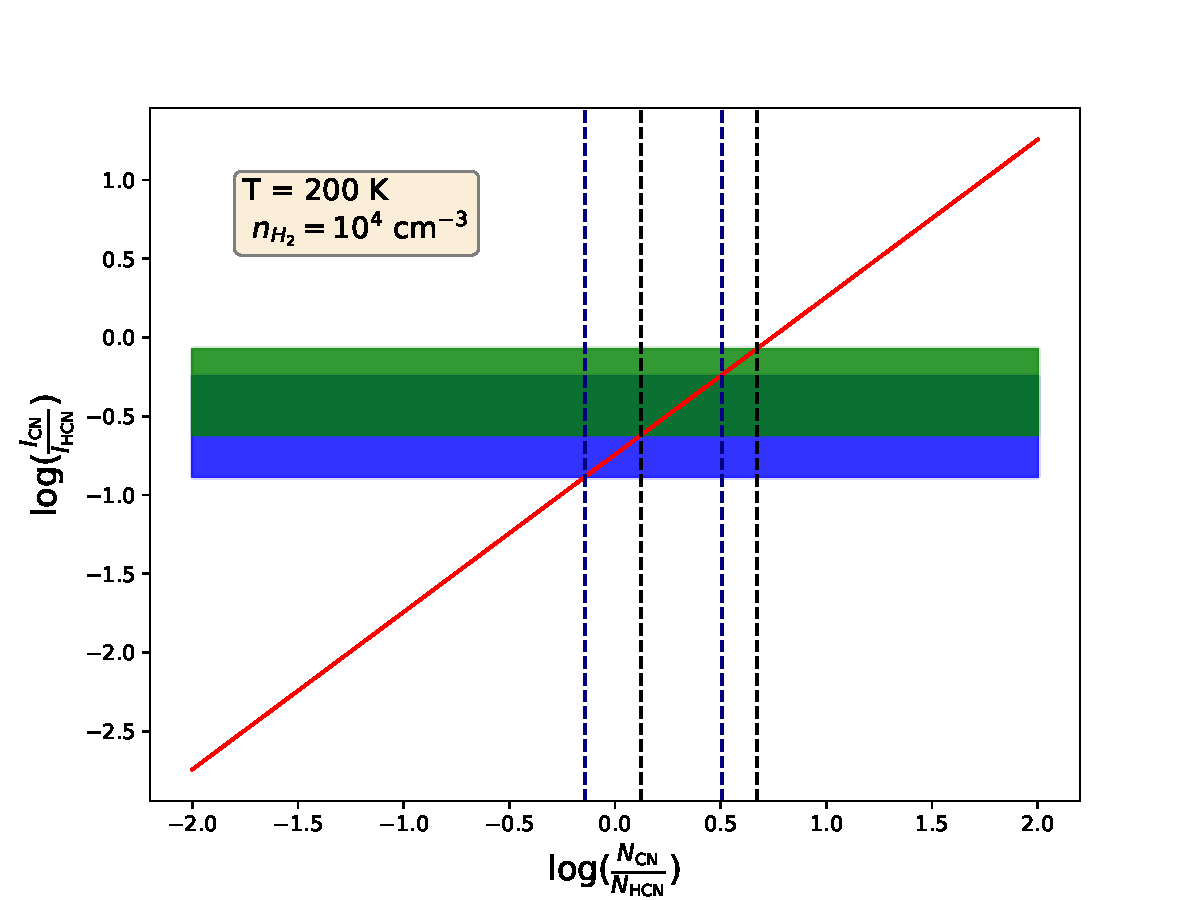
\includegraphics[width=1.\linewidth]{RADEX_CN_HCN_200K_1e4.eps} 
%\caption{}
\end{subfigure}
\begin{subfigure}{.45\textwidth} 
\label{model4} 
\centering
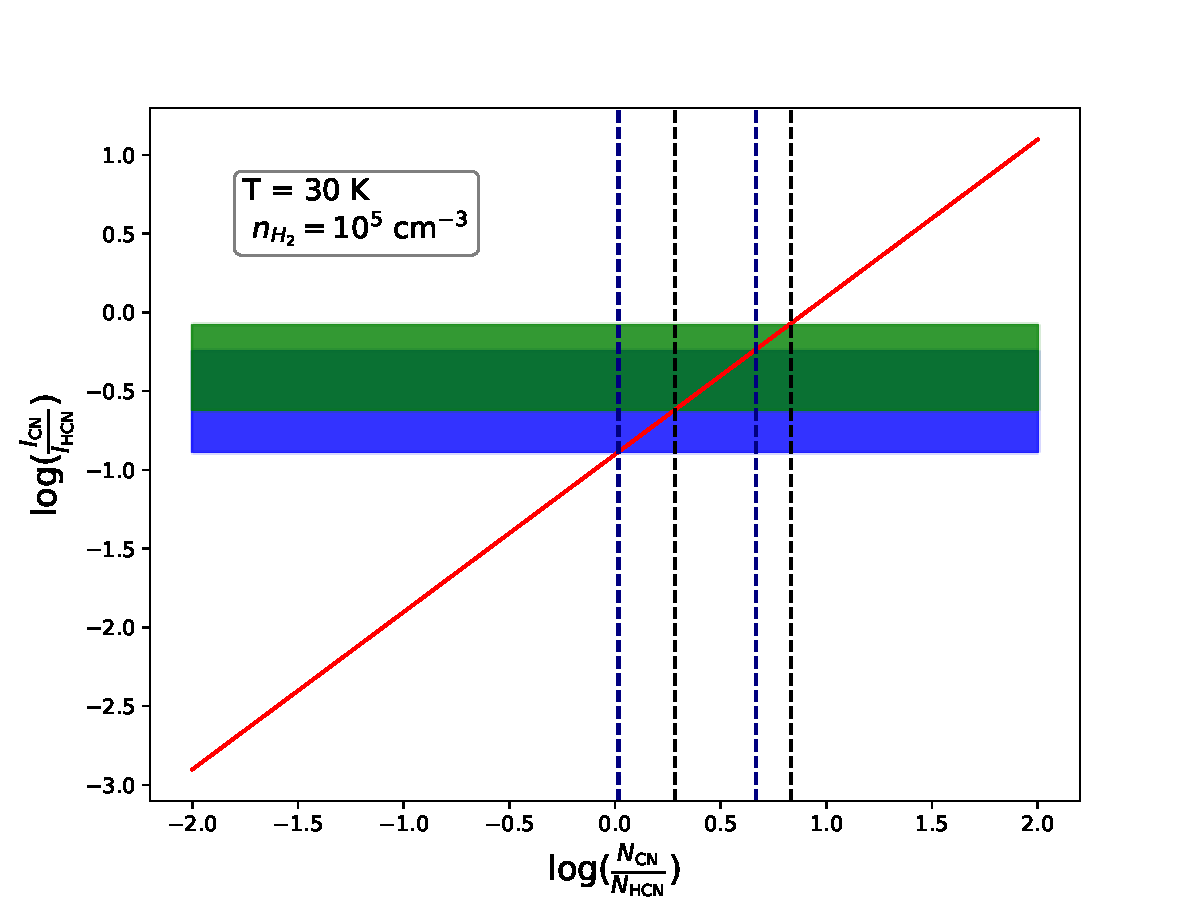
\includegraphics[width=1.\linewidth]{RADEX_CN_HCN_30K_1e5.eps} 
%\caption{} 
\end{subfigure}
\begin{subfigure}{.45\textwidth} \label{model5} 
\centering
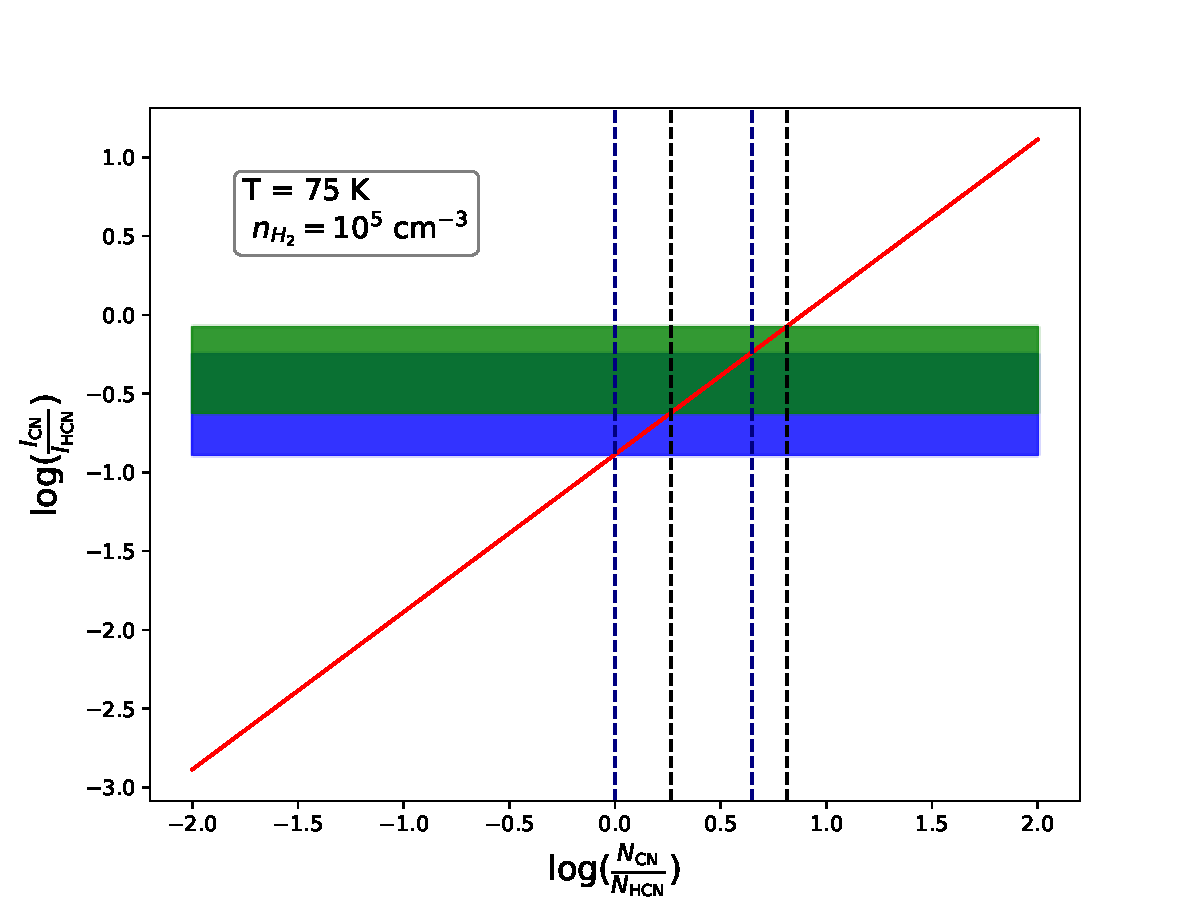
\includegraphics[width=1.\linewidth]{RADEX_CN_HCN_75K_1e5.eps} 
%\caption{} 
\end{subfigure}
\begin{subfigure}{.45\textwidth} 
\label{model6} 
\centering
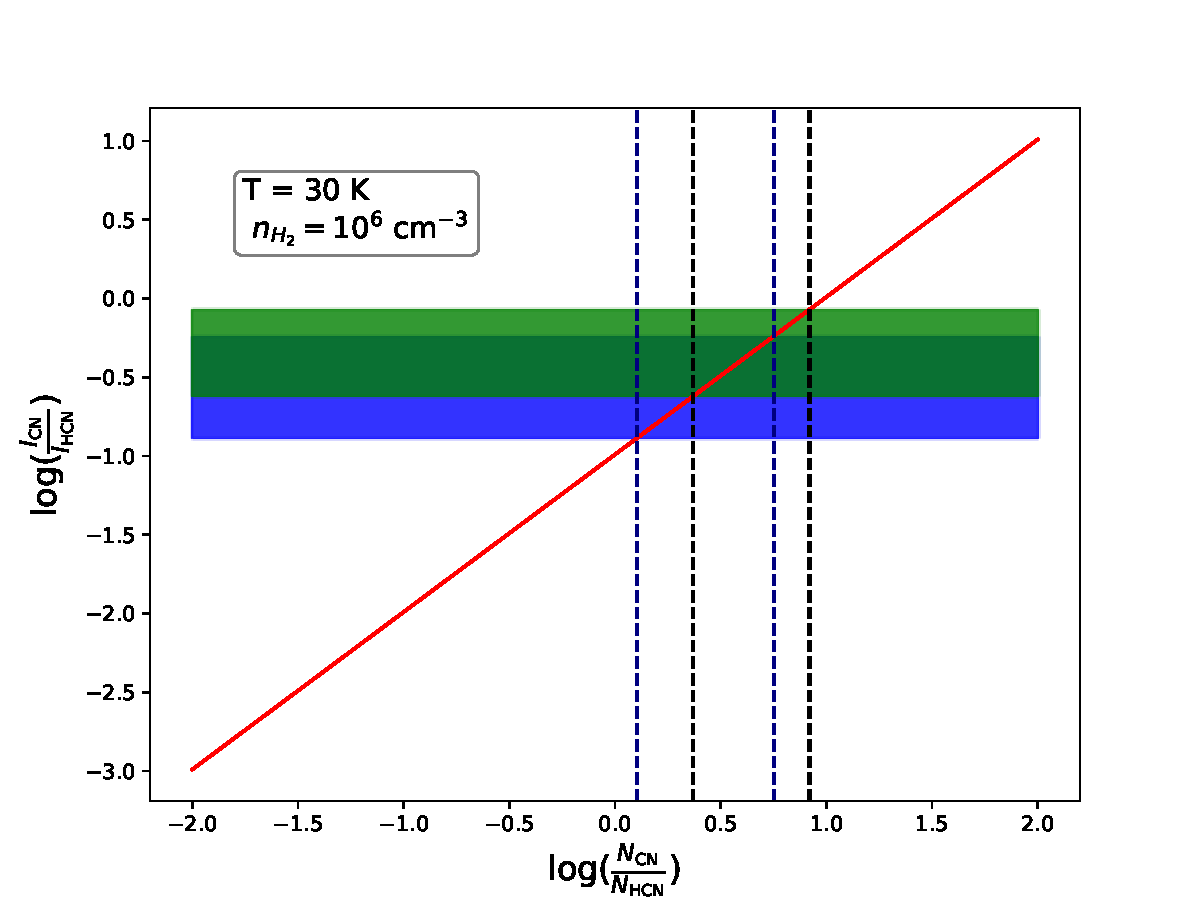
\includegraphics[width=1.\linewidth]{RADEX_CN_HCN_30K_1e6.eps} 
%\caption{} 
\end{subfigure}
\begin{subfigure}{.45\textwidth} 
\label{model7} 
\centering
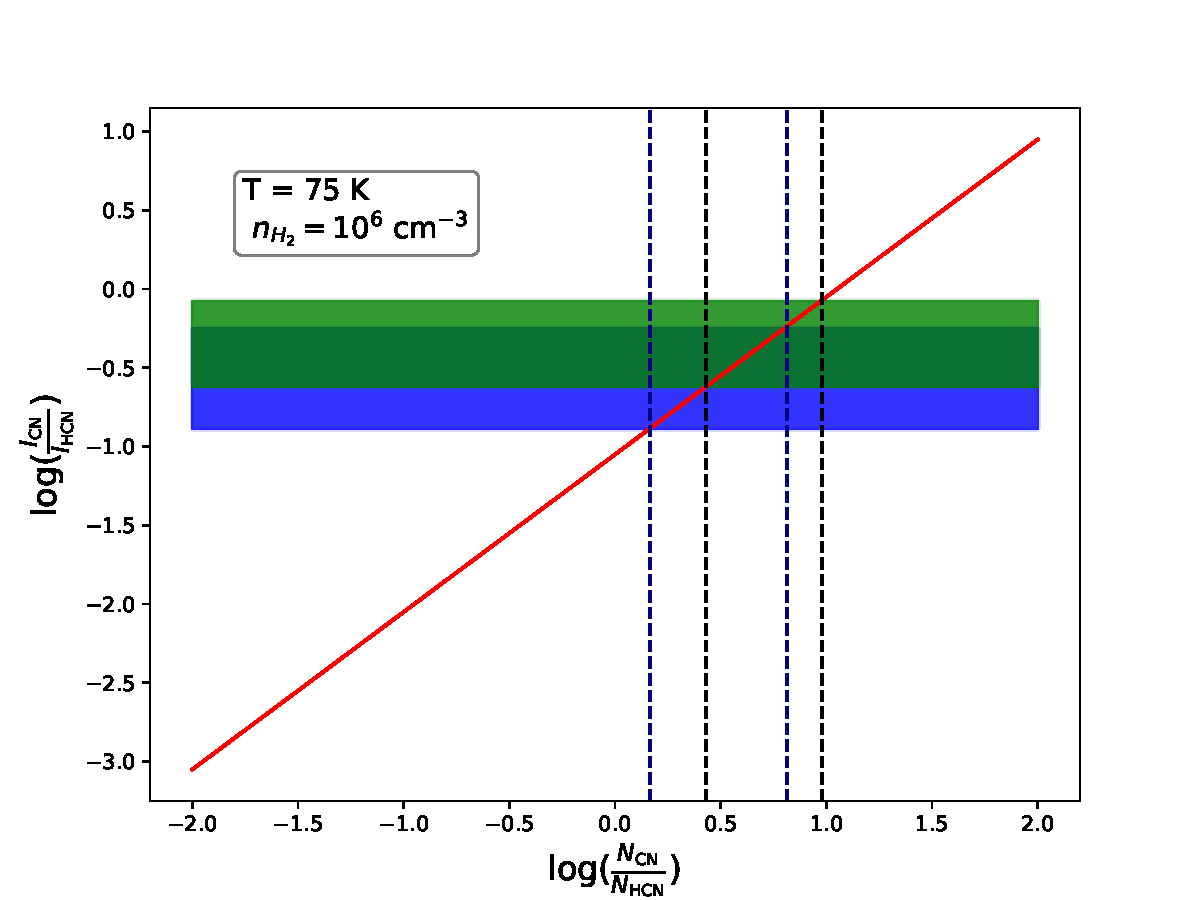
\includegraphics[width=1.\linewidth]{RADEX_CN_HCN_75K_1e6.eps} 
%\caption{} 
\end{subfigure}
\begin{subfigure}{.45\textwidth} 
\label{model8} 
\centering
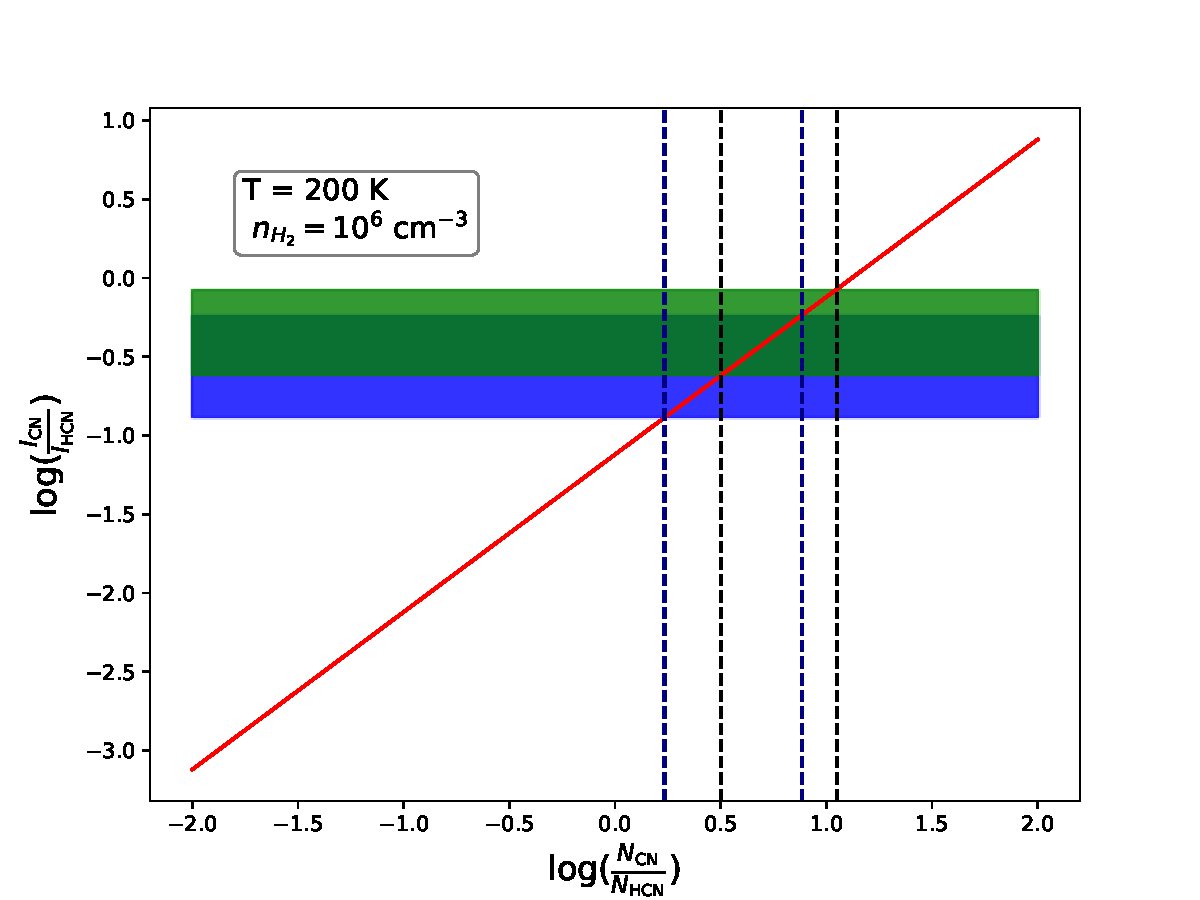
\includegraphics[width=1.\linewidth]{RADEX_CN_HCN_200K_1e6.eps} 
%\caption{} 
\end{subfigure}
\caption{\label{RADEX_models} RADEX models for different parameter. Similar to Fig.~\ref{model}} 
\end{figure*}

\section{Dominant reactions in CN, HCN chemistry}

\textbf{Dominant processes in CN and HCN reactions modelled at the temperature of 50 K are listed in Tab.~\ref{reactions_50}. The processes are illustrated in the Nahoon model parameter space: main channels of HCN and CN destruction, as well as HCN and CN production (Fig.~\ref{HCN_dest} and Fig.~\ref{CN_dest} - Fig.~\ref{CN_prod} respectively). Only the reactions contributing at least 30\% in total flux were taken into consideration. Dominant reactions are more dependent on the strength of the UV radiation than on the hydrogen density. Reaction networks for UV radiation in weak (G$_0$ = $10^{-4} - 10^{-1}$), intermediate (G$_0$ = $10^{-1} - 10^{1}$) and strong (G$_0$ = $10^{1} - 10^{6}$) regime are presented in Fig.~\ref{reactions_smallG0}, Fig.~\ref{reactions_mediumG0} and Fig.~\ref{reactions_largeG0} respectively. Not only the dominant reactions, but also the main route of the reactants production were illustrated. The dominant processes modelled assuming the temperature of 200 K are listed in Tab.~\ref{reactions_200}.}

\begin{table*} 
\caption{Dominant processes in CN, HCN chemistry - outflow (200K)}             %
\label{reactions_200}      % is used to refer this table in the text \centering          
               % used for centering table 
               
\begin{tabular}{c c c c} \hline\hline Molecule & Weak UV fields  & Medium UV fields  & Strong UV fields  \\
& (G$_0$ = $10^{-4} - 10^{-1})$ & (G$_0$ = $10^{-1} - 10^{1})$ & (G$_0$ = $10^{1} - 10^{6})$ \\ 
\hline 
\multirow{8}{*}{CN} & \multicolumn{3}{c}{\textbf{Destruction}}\\
 &O + CN $\rightarrow$ N + CO & CN + ph $\rightarrow$ C + N & CN + ph $\rightarrow$ C + N\\
  &CN + N $\rightarrow$ C + N$_2$ & O + CN $\rightarrow$ N + CO & \\
\vspace{2.5 pt} & \multicolumn{3}{c}{\textbf{Production}}\\ 
&CNC$^+$ + e$^-$ $\rightarrow$ C + CN & N
+ C$_2$ $\rightarrow$ C + CN &  H + CN$^+$ $\rightarrow$ CN + H$^+$\\ 
&N + C$_2$ $\rightarrow$ C + CN & H + CN$^+$ $\rightarrow$ CN + H$^+$ & HCN$^+$ + e$^-$ $\rightarrow$ H + CN \\
&HCN + ph $\rightarrow$ H + CN &  & N + C$_2$ $\rightarrow$ C + CN\\
 &  &   & N + CH $\rightarrow$ H + CN\\ 
 &  &   & HCN + ph $\rightarrow$ H + CN\\ 
 \hline 
 \multirow{9}{*}{HCN} & \multicolumn{3}{c}{\textbf{Destruction}}\\ 
 &HCN + C$^+$ $\rightarrow$ H + CNC$^+$ & HCN + C$^+$ $\rightarrow$ H + CNC$^+$ &  HCN + ph $\rightarrow$ H + CN\\
 &HCN + ph $\rightarrow$ H + CN &HCN + ph $\rightarrow$ H + CN & HCN + C$^+$ $\rightarrow$ H + CNC$^+$\\
 &HCN + HCO$^+$ $\rightarrow$ CO + HCNH$^+$ &  &  \\
\vspace{2.5 pt} &\multicolumn{3}{c}{\textbf{Production}}\\
&N + CH$_2$ $\rightarrow$ H + HCN & H + CCN $\rightarrow$ C + HCN & HCNH$^+$ + e$^-$ $\rightarrow$ H + HCN\\
&H + CCN $\rightarrow$ C + HCN & HCNH$^+$ + e$^-$ $\rightarrow$ H + HCN & H + CCN $\rightarrow$ C +
HCN\\ &CN + H$_2$ $\rightarrow$ H + HCN & & H$_2$NC$^+$ + e$^-$ $\rightarrow$ H + HCN 
\\ &C + HNC$\rightarrow$ C + HCN & & N + CH$_2$ $\rightarrow$ H + HCN \\ 
\hline 
\end{tabular} 
\end{table*}


\begin{figure} 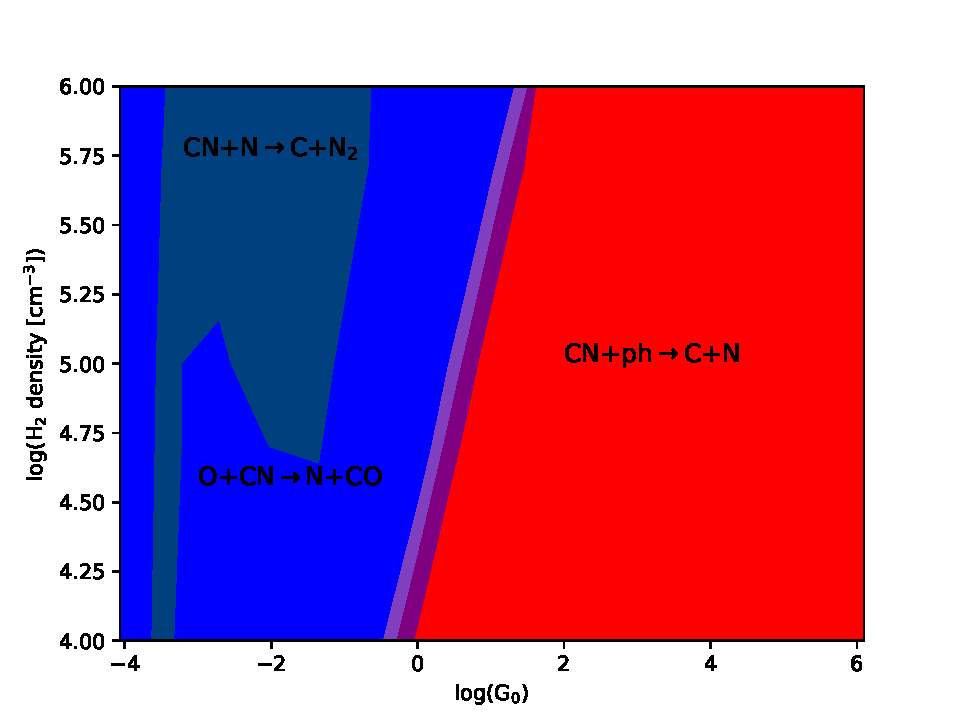
\includegraphics[width=10cm]{destruction_CN_dominant.eps} \caption{Dominant reactions
of CN destruction. Reactions conributed at least 50$\%$ of total flux are marked with full colous.
Transparent colours correspond to 30$\%$-50$\%$ contribution.} \label{CN_dest} \end{figure}

\begin{figure} 
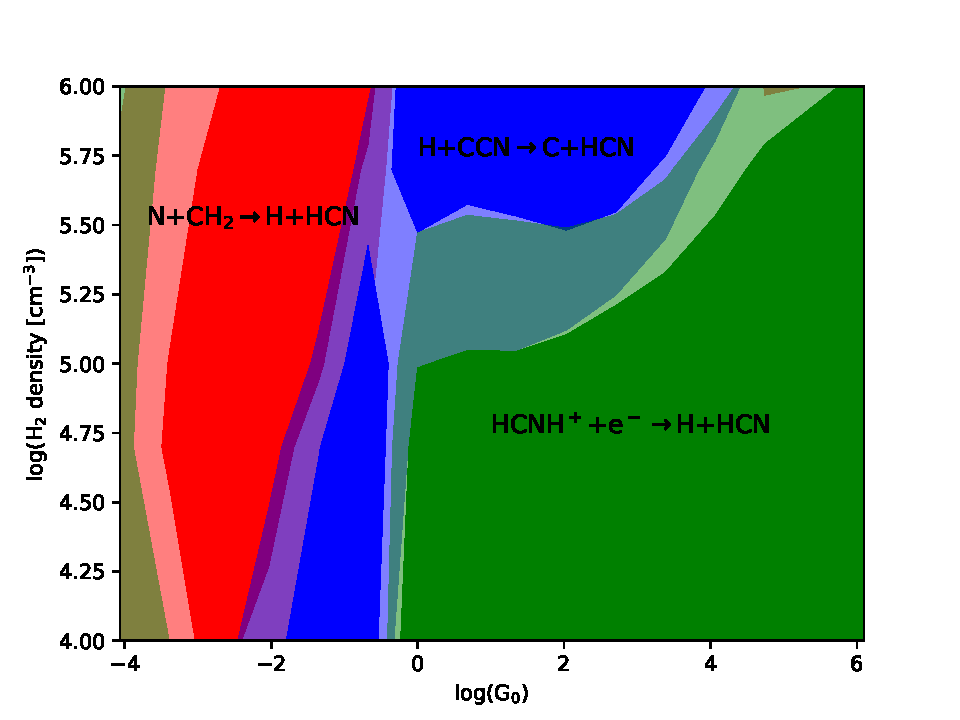
\includegraphics[width=10cm]{production_HCN_dominant.eps} 
\caption{Similar to Fig.~\ref{CN_dest} but for HCN production.} 
\label{HCN_prod} 
\end{figure}

\begin{figure} 
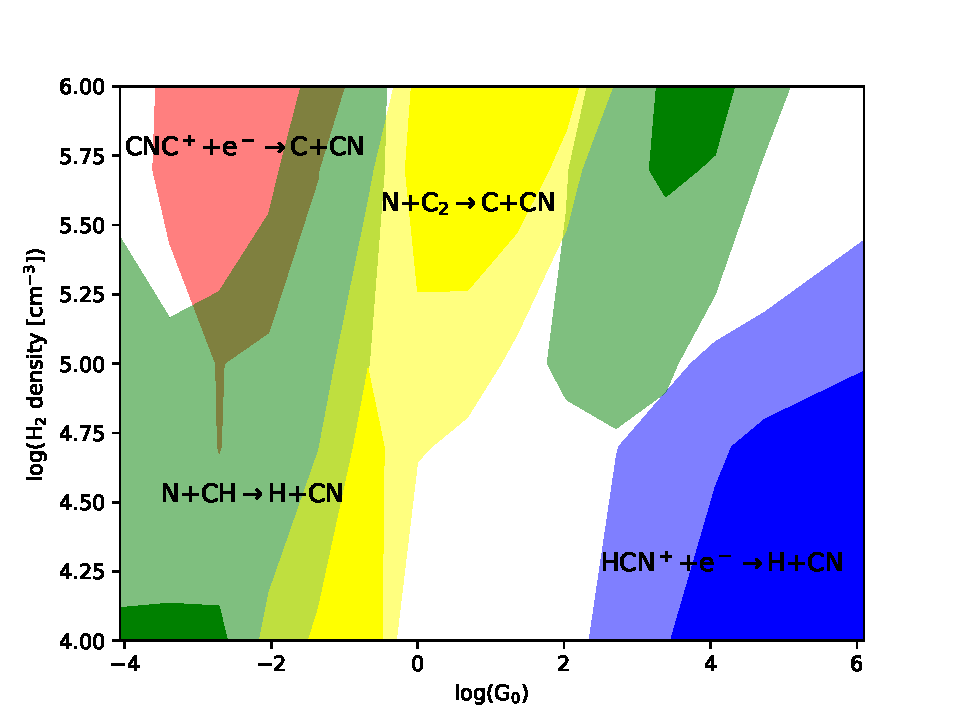
\includegraphics[width=10cm]{production_CN_dominant.eps} 
\caption{Similar to Fig.~\ref{CN_dest} but for CN production.} 
\label{CN_prod}
\end{figure}


\begin{figure} 
\includegraphics[width=10cm]{reactions-smallG0.eps} 
\caption{Reactions network for weakly UV irradiated gas.} 
\label{reactions_smallG0} 
\end{figure}

\begin{figure} 
\includegraphics[width=10cm]{reations_large.eps} 
\caption{Similar to Fig.~\ref{reactions_smallG0} but for for UV field higher than G$_0$ = $10^{1})$.}
\label{reactions_largeG0} 
\end{figure}


\section{Correlations with T$_\mathrm{bol}$ and L$_\mathrm{bol}$} 

\textbf{Fig.~\ref{Tbol_Lbol} compares the luminosity in CN 1-0, HCN 1-0 and CS 3-2 lines in respect to the bolometric luminosities and temperatures of the observed protostars. A molecule luminosity is calculated based on the integrated intensity of a line at 3$\sigma$ level. The integrated flux in K km $s^{-1}$ unit is converted to Jy km $s^{-1}$ using conversion factors Jy/K tabularised in 'Proposals for IRAM Telescopes' document\footnote{www.iram.fr}. Then, Jy is converted to W and divided by the wavelength in km. The luminosity in a line is calculated by the standard relation between luminosity $L$ and flux $F$ (Eq.~\ref{eq8}) and expressed in solar luminosities.}
\begin{equation} 
\label{eq8} 
L = F \; 4 \; \pi \; d^{2}
\end{equation}
\textbf{where distance $d$ is $436 \pm 9.2$ pc (\citealt{Ort17}).}

\hspace*{-1.5in}
\begin{figure*} 
\includegraphics[width=\textwidth]{Lbol_Tbol_correlations.eps} 
\caption{Correlations of lines luminosity with bolometric luminosity and temperature of protostars. Class 0 protostars are marked with red, while Class I with blue colour. The Pearson coefficient of the correlation (r) is shown.}
\label{Tbol_Lbol} 
\end{figure*}


\end{appendix}

\end{document}
%
%%%%%%%%%%%%%%%%%%%%%%%%%%%%%%%%%%%%%%%%%%%%%%%%%%%%%%%%%%%%%%%
%Example below of non-structurated natbib references To use the v8.3 macros with this form of
%composition of bibliography, the option "bibyear" should be added to the command line
%"\documentclass[bibyear]{aa}".
%%%%%%%%%%%%%%%%%%%%%%%%%%%%%%%%%%%%%%%%%%%%%%%%%%%%%%%%%%%%%%
%%%%%%%%%%%%%%%%%%%%%%%%%%%%%%%%%%%%%%%%%%%%%%%%%%%%%%%%%%%%%%
%%%%%%%%%%%%%%%%%%%%%%%%%%%%%%%%%%%%%%%%%%%%%%%%%%%%%%%%%%%%%%
%%%%%%%%%%%%%%%%%%%%%%%%%%%%%%%%%%%%%%%%%%%%%%%%%%%%%%%%%%%%%%
%%%%%%%%%%%%%%%%%%%%%%%%%%%%%%%%%%%%%%%%%%%%%%%%%%%%%%%%%%%%%%
